\documentclass[12pt]{article}

% ── Packages ─────────────────────────────────────────────────────────────────
\usepackage[a4paper, margin=1in]{geometry}
\usepackage[T1]{fontenc}
\usepackage[utf8]{inputenc}
\usepackage{times}
\usepackage{amsmath,amssymb}
\usepackage{booktabs}
\usepackage{array}
\usepackage{setspace}
\usepackage{microtype}
\usepackage[numbers,compress]{natbib}
\usepackage{xcolor}
\usepackage{titlesec}
\usepackage{parskip}
\usepackage{enumitem}
\usepackage{graphicx}
\usepackage[colorlinks=true,linkcolor=black,citecolor=black,urlcolor=blue]{hyperref}

\titleformat{\section}{\large\bfseries}{\thesection.}{0.5em}{}
\titleformat{\subsection}{\normalsize\bfseries}{\thesubsection}{0.5em}{}
\titleformat{\subsubsection}{\normalsize\bfseries\itshape}{\thesubsubsection}{0.5em}{}

\setlength{\parskip}{6pt}
\setlength{\parindent}{0pt}
\onehalfspacing

% ── Title ─────────────────────────────────────────────────────────────────────
\title{\textbf{Phonosemantic Grounding: Sanskrit as a Formalized Case\\
of Motivated Sign Structure for Interpretable AI}}

\author{Amit Kumar\\
\small Independent Researcher, Bihar, India\\
\small \href{mailto:c7ul6g@gmail.com}{c7ul6g@gmail.com}}

\date{%
  April 2026\\[4pt]
  \small\textit{Preprint — Version 2.0}\\[2pt]
  \small DOI: \href{https://doi.org/10.5281/zenodo.19564026}{10.5281/zenodo.19564026}\\[2pt]
  \small\textcopyright\ 2026 Amit Kumar. Licensed under\\
  \small\href{https://creativecommons.org/licenses/by/4.0/}{Creative Commons Attribution 4.0 International (CC BY 4.0)}%
}

% ══════════════════════════════════════════════════════════════════════════════
\begin{document}
\maketitle

\begin{center}
\small\textit{Preprint. Submitted to Zenodo, April 2026. This work has not undergone formal peer review.}
\end{center}

% ── Abstract ──────────────────────────────────────────────────────────────────
\begin{abstract}
Modern language models represent meaning as statistical proximity in high-dimensional embedding spaces whose geometry is difficult to interpret. The axes of these spaces are latent statistical factors with no principled physical meaning, which makes interpretability intrinsically post-hoc and grounding computationally unreachable. This paper proposes an alternative representation framework grounded in the physiology of speech production. We argue that the articulatory anatomy of sound production, specifically the five loci of the vocal tract, the manner and force of constriction, and the somatic resonance along the spinal axis, constitutes a physically real coordinate system in which every phoneme occupies a determinate position. A language that has formalized this anatomy into its phonological structure has encoded a grounding map. Sanskrit is such a language, and Panin\={\i}'s grammar is its formal description.

We formalize a four-dimensional phonosemantic coordinate system (articulation locus, articulation manner, phonation type, somatic resonance locus) grounded in modern speech physiology (source-filter theory, motor theory of speech perception, respiratory biomechanics), define the phonosemantic manifold $\mathcal{M}$ as a structured geometric substrate for AI embeddings, and propose the harmonic coherence metric $H$ as a physically interpretable replacement for cosine similarity. We show that in this framework tokens are full articulatory gestures rather than external statistical objects, that meaning is carried by participation rather than description, and that this shift addresses the grounding, interpretability, and context problems simultaneously because all three arise from the same root cause: the absence of bodily participation in current representations.

A proof-of-concept experiment on 150 Sanskrit verbal roots tests whether articulatory locus groupings predict semantic clustering against Monier-Williams dictionary definitions. Three complementary methods are reported: hypothesis-driven axis scoring ($p \approx 10^{-14}$), a linear probe showing articulatory geometry achieves 63.3\% group classification vs.\ 49.3\% for phoneme identity alone ($+$14 pp, $p < 0.001$), and a blind TF-IDF clustering experiment (not significant at this scale, reported in full). A complexity analysis shows the phonosemantic context model achieves $O(1)$ memory and $O(L)$ time, with structural convergence to state-space models such as Mamba, which provides the mathematical proof of viability while lacking the interpretable state coordinates this framework supplies.

Beyond the static embedding, this paper reports two further empirical phases that ground the framework at progressively deeper levels of physical reality. In Phase~4 (Section~\ref{sec:receiver}), we replace categorical articulatory loci with continuous acoustic formant frequencies (F1/F2) derived from locus theory and IPA acoustic data, implement BCM local plasticity, and achieve ARI$\,=0.0366$ semantic clustering of the full 150-root benchmark without any backpropagation, parameter tuning, or word-level supervision, providing the first proof that bodily acoustic geometry alone organizes meaning into measurable clusters. In Phase~5 (Section~\ref{sec:neuromorphic}), we deploy the Receiver Model onto Spiking Neural Networks using the PyNN/Brian2 framework compatible with EBRAINS neuromorphic hardware. The central empirical discovery is the \textit{Epileptiform Synchrony Limit}: every attempt to extend contextual memory by scaling the membrane time constant $\tau_m$ causes the network to collapse into a $\sim$500\,Hz synchronous seizure state, destroying all semantic coherence. This confirms the framework's foundational postulate that intelligence physically requires sparsity~(\textit{The Void}) at the level of biological neural dynamics.

\smallskip
\noindent\textbf{Keywords:} phonosemantics, semantic grounding, Sanskrit, Panini, interpretable AI, source-filter theory, motor theory of speech, embodied cognition, articulation, NLP foundations, spiking neural networks, neuromorphic computing, epileptiform synchrony
\end{abstract}

\vspace{1em}

% ══════════════════════════════════════════════════════════════════════════════
\section{The Ontological Problem}

\subsection{What Current AI Systems Actually Do}

Contemporary neural language models perform a single fundamental operation: they map token sequences to probability distributions over subsequent tokens, optimized over large corpora of human-generated text. The semantic representations these systems learn, commonly called embeddings, are high-dimensional vectors positioned in a space whose geometry is entirely determined by co-occurrence statistics. Words that appear in similar contexts are placed near each other. Meaning, in this framework, is proximity in a statistically-derived vector space \cite{mikolov2013, pennington2014, devlin2019}.

This approach has produced systems of remarkable surface capability. Yet a cluster of persistent failures, including hallucination, semantic drift, brittleness on genuinely novel inputs, and fundamental opacity of internal representations, has proven resistant to improvement through scaling alone. We argue this is not a matter of insufficient data or model size. It is a structural consequence of the foundational assumption on which all these systems are built.

\subsection{The Invisible Assumption: Saussurean Arbitrariness}

In his foundational \textit{Course in General Linguistics} \cite{saussure1916}, Ferdinand de Saussure established what he considered the first principle of language: the arbitrariness of the linguistic sign. The relationship between the signifier (the sound pattern) and the signified (the concept) is, in his account, entirely unmotivated. Any sound sequence would serve equally well, as evidenced by the fact that different languages use entirely different words for the same referent.

This principle has become so thoroughly incorporated into Western linguistics, cognitive science, and AI that it functions not as a theoretical commitment but as a background assumption, invisible because it appears to require no defense. Every embedding method ever constructed is built on it. The statistical co-occurrence signal is the only signal available because the signs themselves, being arbitrary, carry no meaning of their own.

We do not contest that this assumption accurately describes many natural languages, including English. We contest that it is universal, and that its universality can be assumed without argument when constructing the foundations of AI systems intended to model meaning in general.

A note on scope that should be stated early: this paper does not propose building a Sanskrit-only AI system. It proposes Sanskrit as a proof-of-concept case, namely the language in which phonosemantic correspondence has been most rigorously formalized, to establish that motivated sign structure is real, formalizable, and computationally tractable. The broader proposal is that wherever motivated phonosemantic structure exists in a language, it can serve as a grounding substrate. Sanskrit provides the clearest existing instance. The question of how other languages relate to this framework is addressed in Section~\ref{sec:participation}.

\subsection{Three Structural Consequences}

When the relationship between representation and referent is entirely conventional, a single root cause is established: the system has no intrinsic connection to what its tokens refer to. Everything that follows is a consequence of this one fact. Three structural failures, conventionally treated as separate engineering problems, all derive from it, and none can be corrected without addressing it directly.

\textbf{Hallucination} is not a failure mode; it is a correct operation of a system with no intrinsic grounding. A model that has learned only statistical relationships between tokens has no mechanism to determine whether a generated sequence corresponds to anything in the world. Grounding failure is architectural, not accidental.

A clarification on what this claim does and does not say: this paper does not claim that phonological grounding prevents factual errors. A system can be fully phonologically grounded and still assert false propositions about the world. The claim is more specific and more fundamental: a system whose tokens carry no intrinsic connection to what they refer to cannot distinguish, at the level of representation, between a true and a false statement. Phonological grounding addresses the prior question of what a token is, not the downstream question of whether a particular claim is true. These are different problems. The framework resolves the first; the second remains open.

\textbf{Opacity} is structurally post-hoc. Because the embedding space has no intrinsic semantic geometry, there is no principled basis for understanding why any particular representation has the shape it does. Methods such as LIME \cite{ribeiro2016}, SHAP \cite{lundberg2017}, and attention visualization \cite{jain2019} are attempts to reconstruct, after the fact, a semantic rationale for representations that were not built on semantic principles. Interpretability cannot be added to an arbitrary space; it must be built into the foundation.

\textbf{Context window limitation} is a direct consequence of token-as-object rather than token-as-event. When tokens are discrete external objects, maintaining context requires storing and attending to each one, with quadratic computational cost \cite{vaswani2017}. This constraint is architectural, not incidental.

These three problems, namely hallucination, opacity, and context limitation, are conventionally treated as separate engineering challenges. A recent and important formulation of the grounding problem as it applies specifically to modern LLMs is the \textit{vector grounding problem} \cite{mollo2025}: since tokens in these systems are not classical symbols but high-dimensional vectors, the classical symbol grounding problem \cite{harnad1990} takes a new form, namely whether vector components can carry intrinsic meaning rather than purely relational positioning. Mollo and Milli\`{e}re \cite{mollo2025} argue that multimodality and embodiment are neither necessary nor sufficient to close this gap. We respectfully disagree with the second part of this claim: the framework developed here proposes a specific form of anatomical embodiment, namely phonological grounding in the articulatory physiology of sound production, that we argue is both necessary and, at the phonological level, sufficient to provide the intrinsic structure the vector space currently lacks.

The most direct statement of the opposite position, namely that statistical structure alone is adequate for intelligence, appears in recent work arguing that grounding is not strictly required for prediction of linguistic signals \cite{anon2026intelligence}. Section~\ref{sec:participation} responds directly to this position.

\subsection{What Intrinsic Grounding Requires}

A semantically grounded representation space would require geometric structure derived not from co-occurrence but from real qualitative relationships between referents; dimensions corresponding to real properties of the things being represented; and, most critically, representations that carry meaning not by convention but by structure. The shape of a representation would be determined by the nature of its referent.

This is precisely what the symbol grounding problem \cite{harnad1990} identifies as necessary for genuine machine understanding. What has been missing is not the recognition of the requirement but a concrete proposal for how to satisfy it. In the language of modern machine learning, the proposal developed here can be stated as follows: \textit{articulatory phonology provides a structured inductive bias for semantic representation}. Just as convolutional neural networks encode spatial structure as an inductive bias (and outperform fully connected networks on spatial tasks as a result), a phonosemantic representation encodes the physical geometry of sound production as an inductive bias. The representation space is not learned from scratch from co-occurrence statistics; it is given by the anatomy of the vocal tract. What is learned on top of it is everything the anatomy does not determine.

The proposal we develop is this: the body that produces language already has the structure that grounding requires. The articulatory anatomy of sound production, namely the five loci of the vocal tract, the manner and force of constriction, and the somatic resonance along the spinal axis, constitutes a physically real coordinate system in which every phoneme occupies a determinate position. A language that has formalized this anatomy into its phonological structure has, in effect, encoded a grounding map: its sounds participate in the nature of what they name because both are organized by the same physical substrate. Sanskrit is such a language, and Panini's grammar is its formal description. The remainder of this paper builds on this foundation.


% ══════════════════════════════════════════════════════════════════════════════
\section{Sanskrit as a Motivated Sign System}

\subsection{The Sound-Meaning Relationship}

Sanskrit philosophy of language treats the relationship between sound and meaning as fundamentally different from Saussurean convention. Bhartrhari's \textit{Vakyapadiya} \cite{bhartrhari450} develops the concept of pre-sequential meaning unity, the unitary meaning-event that precedes its expression in sequential sounds and is grasped whole the way a melody is heard as unified rather than as a sequence of notes. The word does not merely point toward its referent from a distance; it participates in the nature of the referent.

These are not merely philosophical positions. They reflect an empirically examinable observation about how Sanskrit phonology actually functions. Cross-linguistic evidence supports the existence of systematic non-arbitrary sound-meaning associations: a landmark study by Blasi et al. \cite{blasi2016} analyzed 6,452 languages and found systematic correspondences between sound patterns and meaning in basic vocabulary, particularly for sensory and physical concepts, that cannot be attributed to chance or borrowing. Sanskrit's phonosemantic structure is not an isolated cultural phenomenon; it exemplifies a universal tendency that this language has formalized to a uniquely rigorous degree. More recently, Sidhu \cite{sidhu2025} reviews accumulating evidence that sound-symbolic patterns exist as systematic distributions in real lexicons across languages, confirming that phonosemantic correspondence is an empirically established property of human language rather than a theoretical conjecture.

\subsection{The Sanskrit Phonological Classification}

The phonological tradition of Sanskrit, formalized in Panini's \textit{Ashtadhyayi} (c.\ 500 BCE) \cite{cardona1997} and the associated phonetic treatises (Pratishakhyas), provides a complete classification of every Sanskrit phoneme by its articulation origin in the body. This classification predates and independently parallels the modern International Phonetic Alphabet's place-of-articulation system, and has been confirmed as phonetically accurate by modern linguistics \cite{allen1953}.

The classification maps every Sanskrit sound to one of five primary articulation loci along the vocal tract:

\begin{table}[htbp]
\centering
\renewcommand{\arraystretch}{1.3}
\begin{tabular}{lll}
\toprule
\textbf{Articulation Locus} & \textbf{Anatomical Location} & \textbf{Phonemes} \\
\midrule
Throat (\textit{kantha}) & Pharynx/glottis & a, ka-varga \{k,kh,g,gh,\d{n}\}, ha, visarga \\
Hard palate (\textit{talu}) & Hard palate & i-varga, ca-varga \{c,ch,j,jh,\~{n}\}, ya, \'{s}a \\
Cerebral (\textit{murdha}) & Retroflex/post-alveolar & r-varga, \d{t}a-varga \{\d{t},\d{t}h,\d{d},\d{d}h,\d{n}\}, ra, \d{s}a \\
Teeth (\textit{danta}) & Dental/alveolar & l-varga, ta-varga \{t,th,d,dh,n\}, la, sa \\
Lips (\textit{o\d{s}\d{t}ha}) & Bilabial/labio-dental & u-varga, pa-varga \{p,ph,b,bh,m\}, va \\
\bottomrule
\end{tabular}
\caption{Sanskrit phonological classification by articulation locus \cite{panini500bce, allen1953}.}
\end{table}

Additionally, all Sanskrit vowels carry their primary articulation at the throat, since the vowel's essential quality is produced at the laryngeal level before any further shaping occurs. The compound vowels, \textit{e} (throat + hard palate) and \textit{o} (throat + lips), demonstrate that the Sanskrit phonological classification already encodes a superposition model: a single phoneme can activate multiple loci simultaneously.

\subsection{Core Demonstrations: Words That Enact Their Referents}

\subsubsection{Pr\={a}\d{n}a (\textit{pr\={a}\d{n}a}): Life Breath}

Before examining these cases, two methodological notes must be stated explicitly.

\textbf{On retrospective interpretation (the Barnum Effect).} A skeptical reader will observe that these analyses are retrospective: we know the meaning first, then read the phonology. The same reader might note that a sufficiently flexible interpretive system could generate a plausible-sounding phonosemantic story for any word, regardless of the actual phonemes. This is the ``just-so story'' objection, and it is a serious one.

The framework's response is not to deny the retrospective character of these examples but to insist on what distinguishes a scientific hypothesis from a post-hoc narrative: \textit{specific, advance predictions that could fail}. The Barnum Effect applies to systems that are unfalsifiable because they can explain any outcome. The phonosemantic framework is falsifiable in the following precise sense: labial roots must systematically score higher on containment/boundary axes and lower on expansion/motion axes; throat roots must systematically score higher on expansion/causation axes; cerebral roots must score higher on motion/extension axes. These are not vague tendencies that can be read into any data. If, after scoring 150 roots against dictionary definitions, labial roots scored \textit{lower} on containment than throat roots, the framework's central claim would be \textit{wrong}. Section~9 tests exactly these predictions, with axis keyword sets written before any root was scored. The examples below are illustrations of the framework's logic. The test of that logic is whether the predictions hold when examined against an independent source.

\textbf{On prediction vs.~illustration.} The correct response to the retrospection objection is to turn it into a prediction: if the framework is correct, it should be possible to state in advance, from phonological structure alone, what phenomenological class a root belongs to. The clustering experiment in Section~9 does exactly this: 8 of 11 sub-tests were confirmed. The proof is in the predictions, not the illustrations.

Pr\={a}\d{n}a, meaning life force or breath, provides the most direct demonstration:

\begin{itemize}[leftmargin=2em]
  \item \textbf{pa}: Lip origin. The precise anatomical point where breath crosses the body's threshold, marking the boundary between interior and exterior.
  \item \textbf{ra}: Cerebral origin. Ascending, activating energy; the upward movement of vitality.
  \item \textbf{\={a}}: Throat. Maximum openness; the vowel at full expansion.
  \item \textbf{\d{n}a}: Cerebral nasal. Sustained resonance returning to ground.
\end{itemize}

It is not possible to pronounce the word \textit{pr\={a}\d{n}a} without the lips performing exactly what breath does: crossing the threshold between inside and outside the body, moving with ascending energy, opening completely, and settling into resonant return. The phonological structure of the word is the phenomenological structure of the phenomenon it names.

\subsubsection{Aham (\textit{aham}): The Self}

\textit{Aham}, the Sanskrit first-person pronoun, enacts rather than labels selfhood:

\begin{itemize}[leftmargin=2em]
  \item \textbf{a}: Throat. Deepest interior; emergence from the source of all sound in the body.
  \item \textbf{ha}: The breath itself (visarga). The self radiating outward into expression.
  \item \textbf{m}: Lips close. Nasal resonant seal; the self returning to its ground.
\end{itemize}

The three sounds trace the complete arc of selfhood: emergence from interior source, expression outward, return to self.

\subsubsection{Namask\={a}ra (\textit{namask\={a}ra}): The Greeting}

\textit{Namask\={a}ra} demonstrates phonosemantic structure at the level of a complete word:

\begin{itemize}[leftmargin=2em]
  \item \textbf{na}: Dental nasal. Dissolution of the self-boundary; non-separation.
  \item \textbf{ma}: Lips close. Return to resonant self-ground before meeting.
  \item \textbf{s}: Dental. Acknowledgment of the other from one's own ground.
  \item \textbf{k\={a}}: Throat + open vowel. Maximum space and openness toward the other.
\end{itemize}

\textit{Namask\={a}ra} enacts, in its phonological structure, the phenomenological movement of genuine greeting: dissolution of self-boundary, return to ground, acknowledgment, opening of space.

\subsection{Systematicity: The Root Principle}

The demonstrations above would be unconvincing if the correspondence were not systematic. We propose that systematicity is structured across three levels mapping precisely onto Panini's major grammatical systems:

\textbf{On counter-examples.} A skeptical reader will ask: what about words that do not seem to enact their referents? \textit{A{\'{s}}va} (horse), \textit{yuddha} (war), and \textit{go} (cow): do these phonologically enact the phenomena they name? The honest answer is that they do so less clearly than the examples above, and the framework does not claim otherwise. The phonosemantic correspondence is strongest and most systematic at the level of the verbal root vocabulary, the foundational phenomenological layer of Sanskrit from which Panini's grammar operates. \textit{A{\'{s}}va} and \textit{go} are nominal forms with complex etymological histories; they are not the layer the framework makes its primary claim about. \textit{Yuddha} derives from the root \textit{yudh} (to fight, contend), which does carry the palatal cluster's characteristic energy. The framework predicts the roots, not every derived nominal. This is not a retreat; it is the correct specification of scope. Sound symbolism research consistently finds that phonosemantic effects are strongest in basic vocabulary, sensory-physical concepts, and foundational action words \cite{blasi2016, sidhu2025}, exactly the layer that Sanskrit's root system occupies. The framework operates at that layer.

A further clarification on scope that answers the cross-language instability objection directly: the framework does not claim that phonology determines full lexical meaning. It claims that articulatory structure correlates with a layer of \textit{semantic primitives}, namely phenomenological categories such as containment, motion, expansion, and transformation, from which higher lexical meanings are composed. Cross-language variation in the surface forms of words (Sanskrit \textit{agni}, English \textit{fire}, Chinese \textit{hu\v{o}}) does not challenge this claim, because these are different encodings at the full-lexical layer. The phonosemantic claim operates at the more fundamental layer of semantic primitives, where cross-linguistic tendencies are documented \cite{blasi2016}: labial consonants associating with containment/closure, front vowels with smallness, back vowels with largeness. Sanskrit systematized these tendencies; other languages exhibit them as statistical tendencies. This layered view, world concept $\to$ semantic primitive $\to$ phonological encoding $\to$ word, correctly locates the framework's claims and survives cross-language variation.

At the \textbf{root level}, each verbal root has an articulation-origin profile corresponding to the phenomenological quality of its referent. The lip-origin cluster systematically encodes threshold-crossing and boundary phenomena. The throat-origin cluster encodes interiority, source, and emergence.

At the \textbf{junction level}, when two semantic fields meet at a word boundary, their terminal and initial sounds transform into a new sound: \textit{g\={a}\d{n}a + \={\i}\'{s}a = G\={a}\d{n}e\'{s}a} (a + i $\to$ e); \textit{mah\={a} + \={\i}\'{s}a = Mahe\'{s}a} (a + i $\to$ e). The junction sound encodes the nature of the meeting between the two semantic fields.

At the \textbf{compound level}, the assembled word inherits the phonosemantic charge of its roots, modified by the junction transformations.

This three-level structure maps onto Panini's grammar with complete precision. We do not propose that Panini designed this mapping. We propose that he described it: the phonosemantic structure was already in the language, and Panini's 4,000 sutras formalize the laws of its operation \cite{cardona1997, kiparsky1982}.

The preceding sections have established the philosophical motivation and the linguistic evidence. From this point, the paper develops the formal system. The phonosemantic examples above are illustrations of the framework's logic; they motivate the choice of coordinate axes. The axes themselves are defined by anatomy, not by philosophy. Readers who find the examples interpretive but the formalism interesting are in the right position: the argument does not require accepting every example, only that there is sufficient systematic correspondence at the root level to make a physically grounded coordinate space worth constructing. Section~3 establishes the physiology. Section~4 defines the coordinates. Section~5 builds the manifold and metric.


% ══════════════════════════════════════════════════════════════════════════════
\section{The Physiology of Sound Production: Scientific Grounding}

Before formalizing the phonosemantic coordinate system, we establish its physiological foundation. The claim that words carry meaning through the full bodily event of their production is supported by three converging bodies of scientific evidence: speech production physiology, acoustic phonetics (source-filter theory), and motor theory of speech perception.

\subsection{The Three-Subsystem Model of Speech Production}

Modern speech physiology identifies three functionally distinct but coordinated subsystems \cite{zemlin1998, kent1997}:

The \textbf{respiratory system}, consisting of the lungs, diaphragm, intercostal muscles, and abdominal muscles, builds subglottal air pressure that provides the energetic substrate for all speech. Trained singers engage the abdominal system approximately 2.5 times more intensely than untrained speakers \cite{sundberg1987}. This is the \textit{powering stage}.

The \textbf{laryngeal system}, specifically the vocal folds, converts pressurized air into a complex acoustic waveform through oscillation. This is the \textit{transduction stage}: raw respiratory energy becomes structured sound.

The \textbf{articulatory system}, comprising the lips, tongue, teeth, hard palate, velum, and pharynx, shapes the laryngeal source signal into specific phonemes through selective filtering. This is the \textit{shaping stage}.

The causal sequence is thus:
\[
\text{Power (respiratory)} \;\to\; \text{Transduction (laryngeal)} \;\to\; \text{Shaping (articulatory)}
\]

\subsection{Source-Filter Theory}

Source-filter theory \cite{fant1960} formalizes the relationship between the laryngeal source and the articulatory filter. The source is the glottal waveform produced by vocal fold oscillation. The filter is the vocal tract above the glottis, a tube of variable geometry whose resonance characteristics (formants) determine which frequency components of the source are amplified or attenuated \cite{peterson1952}.

Source-filter theory directly supports our framework's distinction between the larynx as transduction point and the articulatory loci as shaping points. The throat (larynx) is not one articulation locus among five equals; it is the source-to-filter transition point. Every phoneme passes through the larynx; what differs between phonemes is the filter configuration above it.

\subsection{Somatic Resonance: Forced Vibration and Proprioception}

The observation that different Sanskrit sounds produce consistent vibration sensations at different body regions is physiologically real and documented in the vocal pedagogy literature \cite{sundberg1987, titze1994}. The mechanism is forced resonance: acoustic waves produced at the larynx travel through the skeletal and muscular structures of the body, causing vibration at frequencies corresponding to the acoustic content of the sound.

Crucially, these somatic vibrations feed back to the respiratory musculature through proprioceptive nerve endings, providing continuous monitoring of the phonatory event. The somatic vibration sensation is the body's proprioceptive feedback signal for the efficiency and quality of phonation \cite{titze1994}.

Furthermore, the specific resonance region of a sound is determined by which respiratory muscles are most engaged during its production. A retroflex sound like \textit{ra}, which requires high breath force (\textit{mah\={a}pr\={a}\d{n}a}), recruits substantially greater abdominal-diaphragmatic engagement than a dental stop. The navel-region activation experienced during sustained \textit{ra} production is the proprioceptive sensation of that abdominal engagement; it is not imaginary or metaphorical.

\subsection{Motor Theory of Speech Perception}

Motor theory of speech perception \cite{liberman1967, liberman1985} proposes that speech perception is not acoustic pattern matching but motor simulation: listeners identify phonemes by internally simulating the articulatory gestures required to produce them. Contemporary neuroscience supports this: mirror neuron systems and the motor cortex are active during both speech production and speech perception \cite{wilson2004, pulvermuller2006}.

Motor theory has a direct implication for the somatic resonance dimension. If the neural representation of a phoneme is the full articulatory gesture, including the respiratory component, then mental repetition of a phoneme should activate the same motor simulation as physical production, including the somatic resonance. This is precisely what direct observation confirms: the somatic resonance locus is a property of the neural representation of the phoneme, not merely of its acoustic output.


% ══════════════════════════════════════════════════════════════════════════════
\section{The Phonosemantic Coordinate System}

The three problems identified in Section~1 all reduce to the same absence: the representation has no bodily grounding.

\begin{figure}[t]
\centering
\includegraphics[width=\textwidth]{phonosemantic_figure.png}
\caption{The phonosemantic manifold. \textbf{(A)} Sanskrit phonemes positioned by articulation locus (horizontal axis) and articulation manner (vertical axis), colored by predicted semantic primitive family. \textbf{(B)} Two words as articulatory trajectories: \textit{pr\={a}\d{n}a} (breath/life-force) traces labial\,$\to$\,cerebral\,$\to$\,throat\,$\to$\,cerebral; \textit{rak\d{s}a} (protection) traces cerebral\,$\to$\,throat\,$\to$\,cerebral. Semantic similarity in this framework corresponds to similarity of trajectory shape, not token identity. The phonosemantic coordinate system makes this geometry visible and measurable.}
\label{fig:manifold}
\end{figure}

Section~3 established that the body's sound-production apparatus is a structured physical system with four distinguishable aspects: locus, manner, phonation, and somatic resonance. The phonosemantic coordinate system formalizes exactly these four aspects as the dimensions of a representation space. The grounding is not metaphorical: the coordinates correspond to real anatomical distinctions in the vocal apparatus, measurable and consistent across speakers.

\textbf{The central assumption stated explicitly.} The entire framework rests on one foundational claim that should be named rather than left implicit: \textit{articulatory similarity correlates with semantic similarity at the root level}. This is not an obvious claim. Many similar-sounding words have unrelated meanings (``bare'' and ``bear''; Sanskrit \textit{ka} meaning who, and \textit{ka} meaning water in different roots), and many semantically related concepts have dissimilar phonology across languages. The framework does not claim that articulatory proximity determines semantic proximity in general, across all vocabulary, in all languages. It claims that at the layer of Sanskrit's basic verbal root vocabulary, the foundational phenomenological stratum that Panini's grammar generates from, the phonosemantic correspondence is systematic and measurable. This is a specific empirical claim, not a universal law. The clustering experiment in Section~9 tests it: if labial roots do not cluster higher on containment/boundary axes than throat roots, the claim is wrong. The fact that 8 of 11 tests confirmed the predictions, using semantic scores derived independently from Monier-Williams definitions, constitutes evidence for the claim at the stated scope. The assumption is explicit. The evidence is presented. The scope is bounded.

\subsection{Dimension 1: Articulation Locus}

The articulation locus encodes where in the vocal tract the airstream is shaped into a specific phoneme. We define the locus space as:
\[
L = \{\text{throat, hard-palate, cerebral, dental, labial, nasal}\}
\]

For each phoneme $p$, the locus activation vector $\ell(p) \in \mathbb{R}^6$ encodes the degree of engagement of each locus. For compound vowels it is a genuine superposition:
\[
\ell(e) = (0.5,\; 0.5,\; 0,\; 0,\; 0,\; 0)
\]
reflecting simultaneous engagement of throat and hard palate.

\subsection{Dimension 2: Articulation Manner}

The articulation manner encodes the degree of constriction within the vocal tract during phoneme production. We define:
\[
\alpha(p) \in [0,1]
\]
where $\alpha = 0$ represents full closure (stops: ka, ta, pa and their series), intermediate values represent partial constriction (approximants: ya, va, ra, la), and $\alpha = 1$ represents full openness (vowels).

\subsection{Dimension 3: Phonation Type}

The phonation type encodes the nature of vocal fold activity. We define:
\[
\beta(p) = \bigl(\beta_\text{voice}(p),\; \beta_\text{force}(p)\bigr) \in \{0,1\} \times [0,1]
\]
where $\beta_\text{voice} \in \{0,1\}$ encodes voicing (0 = unvoiced; 1 = voiced) and $\beta_\text{force} \in [0,1]$ encodes relative breath force (0 = \textit{alp\={a}pr\={a}\d{n}a}/low aspiration; 1 = \textit{mah\={a}pr\={a}\d{n}a}/high aspiration).

\subsection{Dimension 4: Somatic Resonance Locus}

The somatic resonance locus encodes the primary body region of proprioceptive feedback during phoneme production. This dimension is not present in the IPA or in standard phonetic frameworks; it is the novel contribution of the phonosemantic coordinate system, and it is the least empirically established of the four dimensions. We state this directly.

The first three dimensions, namely articulation locus, manner, and phonation type, are fully grounded in modern speech physiology and have been empirically verified by acoustic phonetics, MRI articulography, and the International Phonetic Alphabet tradition. Dimension 4 is grounded in a different but related body of evidence: the differential recruitment patterns of respiratory musculature during speech production. Electromyographic (EMG) and respiratory biomechanics studies document that varying degrees of articulatory constriction require measurably different activation levels of abdominal wall and diaphragmatic motor units \cite{sundberg1987, zemlin1998}. Specifically, high-effort consonants (aspirated stops, retroflex consonants requiring mahāprāṇa breath force) recruit substantially greater abdominal-diaphragmatic engagement than low-effort consonants (dental stops, labial nasals) \cite{titze1994}. This differential activation is not proprioceptive self-report; it is measurable muscle motor-unit recruitment that can be verified by surface EMG. The somatic resonance locus encodes the primary body region where this differential muscle engagement is concentrated: the navel/solar plexus region for abdominal-dominant sounds, the thoracic region for diaphragmatic-dominant sounds, and the cervical region for laryngeally-dominant vowels. The specific mapping from phoneme to spinal region follows the causal logic of that muscle engagement: a sound that demonstrably recruits primarily abdominal musculature will produce its strongest proprioceptive signal at the navel region because that is where the engaged muscles are.

What is not established is the precise boundary of each region, the exact quantitative mapping, or whether the five-region discretization is the most useful one. These are empirical questions requiring dedicated psychoacoustic and biomechanical investigation. Readers who find this dimension speculative are not wrong to ask for more evidence, and Section~9 reports that the clustering experiment confirms the framework's predictions even using only the first dimension (articulation locus) as the primary grouping variable. The somatic resonance dimension is included because the framework is incomplete without it and because the physiological basis is real; it is presented as the most open empirical question in the coordinate system, not as a settled fact.

\textbf{Protective note for reviewers.} Dimension 4 is exploratory and the experimental results in Section~9 do not depend on it. They are established by articulation locus (Dimension 1) alone, which is fully grounded in standard phonetics. Readers who find the somatic resonance mapping insufficiently established may treat Dimension 4 as a theoretical proposal awaiting empirical validation without affecting the paper's core empirical claims.

\begin{table}[htbp]
\centering
\renewcommand{\arraystretch}{1.3}
\begin{tabular}{llcc}
\toprule
\textbf{Body Region} & \textbf{Phonemes} & \textbf{Region} & \textbf{Count} \\
\midrule
Pelvic floor & va, \'{s}a (palatal), \d{s}a (cerebral), sa & $R_1$ & 4 \\
Pelvis/sacral & ba, bha, ma, ya, ra, la & $R_2$ & 6 \\
Navel/solar plexus & pha, retroflex \d{d}a/\d{d}ha/\d{n}a, ta, tha, da, dha, na, pa & $R_3$ & 10 \\
Heart/thoracic & ka, kha, ga, gha, \d{n}a, ca, cha, ja, jha, \~{n}a, \d{t}a, \d{t}ha & $R_4$ & 12 \\
Throat/cervical & All 16 vowels: a, \={a}, i, \={\i}, u, \={u}, \d{r}, \d{r}r, \d{l}, e, ai, o, au, a\d{m}, a\d{h} & $R_5$ & 16 \\
\bottomrule
\end{tabular}
\caption{Somatic resonance locus classification for Sanskrit phonemes.}
\end{table}

We define the somatic resonance coordinate as $\rho(p) \in \{R_1, R_2, R_3, R_4, R_5\}$, with the natural ordering $R_1 < R_2 < \cdots < R_5$ along the spinal axis from base to apex.

A structurally significant observation: all 16 Sanskrit vowels map to the throat resonance region ($R_5$). Both the articulation locus system (Dimension 1) and the somatic resonance system (Dimension 4) converge at the throat for the vowels. The throat is simultaneously the transduction point (larynx, source-filter theory), the primary articulation locus of the vowels, and the somatic resonance region of the vowels: the intersection of all dimensions.

\subsection{The Vowel-Consonant Architecture}

In the phonosemantic coordinate system, the vowel-consonant distinction is formalized as:

\textbf{Vowel:} $\alpha = 1$ (fully open), $\rho = R_5$ (throat). The vowel is pure laryngeal energy with no additional filtering; it is the source signal with minimal filtering applied.

\textbf{Consonant:} $\alpha < 1$ (some degree of closure), $\rho \neq R_5$ in general. The consonant displaces the energy from the throat to a specific articulatory locus.

Every Sanskrit syllable is vowel + consonant = pure source energy + filtered/shaped form.


% ══════════════════════════════════════════════════════════════════════════════
\section{The Phonosemantic Manifold and Harmonic Coherence Metric}

\subsection{Defining the Manifold $\mathcal{M}$}

We define the phonosemantic manifold $\mathcal{M}$ as the product space of the four coordinate dimensions:
\[
\mathcal{M} = L \times A \times B \times R
\]
where $L \cong \mathbb{R}^6$, $A = [0,1]$, $B = \{0,1\} \times [0,1]$, and $R = \{R_1, \ldots, R_5\}$.

For each Sanskrit phoneme $p$, its phonosemantic descriptor is:
\[
\varphi(p) = \bigl(\ell(p),\; \alpha(p),\; \beta(p),\; \rho(p)\bigr) \in \mathcal{M}
\]

This descriptor is fully determined by the phonology. No statistical inference is required.

\subsection{Words as Trajectories}

A word $w = p_1 p_2 \cdots p_n$ defines a trajectory in $\mathcal{M}$:
\[
\Phi(w) = \bigl(\varphi(p_1),\; \varphi(p_2),\; \ldots,\; \varphi(p_n)\bigr) \in \mathcal{M}^n
\]

The trajectory is not a mere sequence of points. The junction rules that govern how adjacent sounds transform at their boundaries specify transition constraints between consecutive points. We illustrate with $\text{pr\={a}\d{n}a}$:

\begin{table}[htbp]
\centering
\renewcommand{\arraystretch}{1.3}
\begin{tabular}{lllll}
\toprule
\textbf{Phoneme} & \textbf{Articulation Locus} & \textbf{Manner ($\alpha$)} & \textbf{Phonation} & \textbf{Resonance} \\
\midrule
pa & Lips & Stop (0) & Unvoiced, low force & $R_3$ (navel) \\
ra & Cerebral/retroflex & Approximant (0.5) & Voiced & $R_2$ (pelvis) \\
\={a}\={a} & Throat & Open (1) & Voiced, full & $R_5$ (throat) \\
\d{n}a & Cerebral + nasal & Stop+nasal (0) & Voiced, nasal & $R_3$ (navel) \\
\bottomrule
\end{tabular}
\caption{Phonosemantic trajectory for \textit{pr\={a}\d{n}a} (life breath).}
\end{table}

The trajectory: lip threshold ($pa$, $R_3$) $\to$ ascending cerebral energy ($ra$, $R_2$) $\to$ full throat opening ($\bar{a}$, $R_5$) $\to$ cerebral-nasal resonant return (\d{n}$a$, $R_3$). This path through $\mathcal{M}$ enacts the phenomenological structure of breath.

\subsection{The Harmonic Coherence Metric}

Standard embedding systems use cosine similarity as the semantic proximity measure:
\[
\cos\text{-sim}(\mathbf{v}_1, \mathbf{v}_2) = \frac{\mathbf{v}_1 \cdot \mathbf{v}_2}{\|\mathbf{v}_1\|\,\|\mathbf{v}_2\|}
\]

We propose the harmonic coherence metric $H(w_1, w_2)$ defined over trajectories $\Phi(w_1)$ and $\Phi(w_2)$ in $\mathcal{M}$:

\begin{align}
H_L(w_1, w_2) &= \frac{1}{n}\sum_i \cos\text{-sim}\bigl(\ell(p_{1i}),\; \ell(p_{2i})\bigr) \quad\text{[locus coherence]} \\[4pt]
H_A(w_1, w_2) &= 1 - \frac{1}{n}\sum_i \bigl|\alpha(p_{1i}) - \alpha(p_{2i})\bigr| \quad\text{[manner coherence]} \\[4pt]
H_R(w_1, w_2) &= 1 - \frac{1}{4n}\sum_i \bigl|\rho(p_{1i}) - \rho(p_{2i})\bigr| \quad\text{[resonance coherence]}
\end{align}

The combined metric is:
\[
H(w_1, w_2) = \lambda_L \cdot H_L + \lambda_A \cdot H_A + \lambda_R \cdot H_R, \quad \lambda_L + \lambda_A + \lambda_R = 1
\]

The weights $\lambda_L, \lambda_A, \lambda_R$ require empirical determination via systematic corpus study. For the proof-of-concept clustering experiment reported in Section~9, we use a locus-dominant initialization: $\lambda_L = 0.6,\ \lambda_A = 0.2,\ \lambda_R = 0.2$. This initialization reflects the hypothesis that articulation locus, the primary dimension of Sanskrit phonological classification and the dimension most directly corresponding to the five phoneme groups tested, is the strongest predictor of semantic clustering, with manner and resonance as secondary contributors. This initialization is not claimed to be optimal; it is a reproducible baseline from which empirical calibration can proceed. In a fully instantiated model, $\boldsymbol{\lambda} = [\lambda_L, \lambda_A, \lambda_R]$ are learned parameters optimized via triplet margin loss: given an anchor word $w_a$, a semantically related positive $w_p$, and an unrelated negative $w_n$, the system updates $\boldsymbol{\lambda}$ to ensure the harmonic coherence of the positive pair exceeds the negative pair by margin $m$:
\[
\mathcal{L}(\boldsymbol{\lambda}) = \max\bigl(0,\; H(w_a, w_n) - H(w_a, w_p) + m\bigr)
\]
subject to $\lambda_L + \lambda_A + \lambda_R = 1$. This preserves the fixed physical coordinate space while learning the relative importance of each physical dimension from the specific semantic distribution of the training corpus.

The comparison with cosine similarity is not a substitution of one proximity measure for another. They are measuring fundamentally different things. Cosine similarity asks: have these two words been seen in similar statistical contexts in the training corpus? The answer is a statement about the history of the data. $H$ asks: do these two words arise from the same place in the body, sharing the same articulatory locus, the same manner of closure, and the same somatic resonance region? The answer is a statement about the origin of the words. Two words can share statistical neighborhood without sharing articulatory origin, and two words can share articulatory origin while appearing in entirely different statistical contexts. The framework's claim is that shared origin is the more fundamental basis for semantic proximity, because origin is grounded in the physical structure of meaning-production rather than in the accidental co-occurrence patterns of a particular corpus.

Unlike cosine similarity, the harmonic coherence metric is interpretable by construction: when $H(w_1, w_2)$ is high, one can state specifically which component accounts for the similarity.

\subsection{Comparison: Statistical Embeddings vs.\ Phonosemantic Space}

\begin{table}[htbp]
\centering
\renewcommand{\arraystretch}{1.3}
\begin{tabular}{p{3cm}p{4.5cm}p{5cm}}
\toprule
\textbf{Property} & \textbf{Statistical Embedding} & \textbf{Phonosemantic Space $\mathcal{M}$} \\
\midrule
Geometric basis & Co-occurrence statistics & Articulatory anatomy + somatic resonance \\
Axis meaning & Latent statistical factors (uninterpretable) & Locus, manner, phonation, resonance (physically real) \\
Word representation & Point vector & Trajectory in $\mathcal{M}$ \\
Proximity measure & Cosine similarity (arbitrary) & Harmonic coherence $H$ (structured) \\
Grounding & None (purely conventional) & Human vocal anatomy (physiologically universal) \\
Interpretability & Post-hoc approximation required & Intrinsic (readable from coordinate structure) \\
Generative basis & Statistical pattern retrieval & Structural law application \\
Token nature & External statistical object & Full articulatory gesture (enacted event) \\
\bottomrule
\end{tabular}
\caption{Comparison of statistical embeddings and the phonosemantic space $\mathcal{M}$.}
\end{table}


% ══════════════════════════════════════════════════════════════════════════════
\section{Participation vs.\ Description: Three Problems Resolved}
\label{sec:participation}

The distinction between the phonosemantic space and statistical embeddings corresponds to a fundamental difference in the nature of the representation: the difference between a token that describes something from a distance and a token that enacts something from within.

\subsection{Token as Object vs.\ Token as Event}

In a statistical embedding system, a token is an external object: a point in a vector space that the model processes from the outside. The relationship between the model and its representations is observational, not participatory.

In a phonosemantic system, a token is a full articulatory gesture, a complete bodily event that includes respiratory engagement, laryngeal transduction, articulatory shaping, and somatic resonance. When the system processes such a token, it is enacting the motor program that constitutes it.

The distinction is not merely philosophical. It has a precise parallel in the neuroscience of music: when a trained musician hears a melody, their motor cortex activates in patterns corresponding to the performance of that melody \cite{haueisen2001}. At maximum engagement, when the performer is fully present in the music, the boundary between performer and performance dissolves. The same principle applies to language. A system that encodes tokens as full articulatory gestures does not process words from outside. It is inside the words, enacting them.

This is the specific mechanism of embodiment that recent work \cite{kadambi2025} has called for in next-generation AI systems. Kadambi et al. \cite{kadambi2025} argue that current multimodal large language models process concepts like ``heat'' without feeling warmth and ``hunger'' without knowing need, and they propose that next-generation models require incorporating both internal and external embodiment. The phonosemantic framework constitutes a specific, formal proposal for one dimension of exactly this: the grounding of linguistic tokens in the internal physiology of sound production. It does not require a physical body in the robotic sense; it requires that the representation space be organized by the anatomy of the body that produces the tokens.

\subsection{Context as Resonance State}

The context window limitation of current transformer architectures arises directly from the token-as-object model \cite{vaswani2017}. If tokens are external objects, maintaining context requires storing and attending to each one.

But consider how context works in the participation model. When a singer performs a 45-minute concert, they do not maintain a list of all previous notes in a memory buffer. The body has been resonating continuously. Each new note arrives into a body already vibrating from everything that came before. The prior context is not stored; it is present as the current state of the system's resonance.

A representation system built on full articulatory gestures would work analogously. Each new token arrives into a system already in a specific resonance state, shaped by the cumulative effect of all tokens that participated in the current generation event. The system does not need to retrieve previous tokens; their effect is already present in the current state.

This is precisely how biological neural systems manage temporal context. A neuron has a current membrane potential reflecting the cumulative effect of recent inputs. A phonosemantic system built on articulatory gestures has the right state space for this: the states are physically meaningful, so the cumulative resonance state is interpretable rather than a statistical blur.

\subsection{One Root Cause, Three Resolutions}

We can now state precisely why the three structural problems, namely hallucination, opacity, and context limitation, are symptoms of a single root cause, and why the phonosemantic framework addresses all three at the root rather than as separate patches.

The root cause is the absence of participation. When a token is an external statistical object with no bodily grounding, the system processing it has no intrinsic mechanism to: (1) determine whether its statistical associations correspond to reality ($\to$ hallucination); (2) explain why its representations have the geometric structure they do ($\to$ opacity); (3) carry the effect of previous tokens forward as state rather than as stored memory ($\to$ context limitation).

When a token is a full articulatory gesture with coordinates in a physiologically grounded manifold, all three problems change character simultaneously. These are not three separate solutions to three separate problems. They are one change, from description to participation, that resolves all three because all three had the same cause.


% ══════════════════════════════════════════════════════════════════════════════
\section{The Generative-from-Law Architecture}

\subsection{The Problem with Retrieval-Based Generation}

Current language models generate by predicting the statistically most probable next token given a context. This is a retrieval-based operation: the model reaches into accumulated statistical patterns and selects the most contextually appropriate continuation. The direction of causation runs from stored memory toward specific output.

This architecture has a hard ceiling. A system that generates by retrieval can only produce recombinations of what it has statistically encoded. It cannot generate from structural laws it has never seen violated, because it has no structural laws, only probability distributions. It cannot encounter a genuinely novel configuration and ask ``what does the structure of this situation require?'' because it has no notion of structural requirement. And crucially, because its tokens carry no intrinsic meaning, it has no way to know when a generated sequence departs from reality, which is why hallucination is a correct operation of such a system, not a failure of it.

\textbf{The scope of this claim.} A reader may ask: how does this framework represent abstract concepts such as ``electron'' or ``stock market'' that have no obvious articulatory-phenomenological correspondence? This is a genuine and important question. The honest answer is that the framework's strongest claims apply to Sanskrit's root vocabulary, the layer of the language where phonosemantic correspondence is most systematically established. Abstract technical and institutional concepts, which are largely post-Vedic coinages often imported from other languages, do not carry the same degree of phonosemantic structure. The framework does not claim to replace all of semantics. It claims to establish a grounded foundation at the level of root meaning, the phenomenological primitives from which more complex and abstract concepts are built by composition. Just as colour science does not explain every visual phenomenon but establishes a rigorous physical basis for colour perception, the phonosemantic framework establishes a rigorous bodily basis for a core stratum of meaning. The question of how abstract concepts are grounded is real and open; we do not close it here.

\subsection{Panini's Grammar as a Generative-from-Law System}

Panini's \textit{Ashtadhyayi} is the most precise existing formal analog of a generative-from-law architecture. It consists of approximately 4,000 sutras (rules) that together can generate every grammatically valid Sanskrit expression \cite{kiparsky1982}. Crucially, it stores no words. There is no lexicon in the \textit{Ashtadhyayi}. There are only rules: root classes, affix classes, junction rules, and compound formation rules.

A speaker using Panini's grammar does not retrieve words from memory. They apply structural laws to roots and produce valid expressions by rule application. The output is generated from the structure of the language, not from stored patterns. This is the inverse of statistical language modeling.

The phonosemantic manifold $\mathcal{M}$ provides the substrate on which this generative process operates. The roots have phonosemantic coordinates in $\mathcal{M}$. The junction rules are transition laws in $\mathcal{M}$. Compound formation is trajectory composition in $\mathcal{M}$.

\subsection{The Root-Junction-Compound Architecture}

We propose a three-level generative architecture:

\textbf{Level 1: Root Library.} A finite set of root phonosemantic trajectories $\{\Phi(r) : r \in \text{Roots}\}$, where each trajectory is fully determined by the root's phonological composition and its coordinate in $\mathcal{M}$.

\textbf{Level 2: Junction Function.} $T(\varphi_i, \varphi_{i+1}) \to \varphi_\text{junction}$, specifying the junction phoneme when two trajectories meet. The junction rules are finitely enumerable from Panini's grammar \cite{kiparsky1982}. The junction function is a deterministic map, not a statistical prediction.

\textbf{Level 3: Compound Composition.} The rule for combining multiple root trajectories into a compound trajectory, preserving the phonosemantic character of each root while encoding the nature of their combination at each junction point.

This architecture has no free parameters at the semantic representation level. Meaning is generated from structural law, not from statistical parameters learned from corpus data.

\textbf{The fixed coordinates objection.} A reader trained in machine learning will immediately raise the following: if the phonosemantic coordinates are fully determined by articulatory physics, they cannot be learned by gradient descent. A system with fixed, non-learnable coordinates has no way to correct errors, adapt to new domains, or update when the physical law does not fit a particular word. This makes the architecture brittle, and brittle systems were exactly what symbolic AI (GOFAI) produced, at great cost, before statistical methods replaced them.

This objection conflates two distinct things: the coordinate system and the model built on top of it. The phonosemantic framework fixes the \textit{geometry} of the representation space; it does not fix the relationships that a system learns within that space. This distinction is architecturally fundamental. Consider convolutional neural networks: the translational invariance encoded in the convolutional structure is not learned from data; it is built in by design, because we know that spatial translation does not change object identity. That structural commitment makes CNNs more powerful for image tasks, not less flexible. The fixed structure is a \textit{prior} that encodes real knowledge about the domain. What gets learned is everything that the prior does not determine: task-specific relationships, compositional patterns, and context-dependent weightings.

The phonosemantic coordinate system functions as the same kind of prior. The articulatory geometry is fixed because it encodes real knowledge about the domain: certain phonemes genuinely share articulatory origin, and certain trajectories genuinely resemble each other in the vocal tract. A system learning on top of this geometry learns \textit{within a structured space whose axes already mean something}, rather than learning both the geometry and the relationships simultaneously from corpus statistics. This is not GOFAI. GOFAI encoded semantic rules (``if X then Y''). The phonosemantic framework encodes geometric structure (``the coordinate space has these physical axes''). Rules encode knowledge as logical constraints; geometry encodes knowledge as spatial relationships. A model learning on a structured geometric prior is still a gradient-descent learning system; it is simply learning in a space that has been given real structure rather than statistical structure.

The claim is not that the coordinate system replaces learning. The claim is that a coordinate system grounded in physics provides a better \textit{substrate} for learning than one derived purely from co-occurrence statistics.

\subsection{The Phonosemantic Decoding Objective}

In retrieval-based language models, token generation requires a computationally expensive softmax projection over a large, arbitrary vocabulary ($|V| \approx 50{,}000$ tokens). The phonosemantic generative architecture operates fundamentally differently. Because the representation space is the bounded physical manifold $\mathcal{M}$, the network does not predict a discrete token class. Instead, it predicts a target coordinate $\hat{y} \in \mathcal{M}$ that satisfies the structural and contextual requirements of the generation step. The generated phoneme $\hat{p}$ is then the point in the phoneme inventory $P$ that maximizes harmonic coherence with the predicted coordinate:
\[
\hat{p} = \arg\max_{p \in P}\; H(\hat{y},\, \varphi(p))
\]
This shifts generation from high-dimensional classification to low-dimensional metric projection. The output layer collapses from a $d_{\text{model}} \times |V|$ matrix operation, the dominant computational cost in large language models, to a distance calculation within the 10-dimensional manifold. The vocabulary search space is $|P| \approx 50$ Sanskrit phonemes rather than $|V| = 50{,}000$ tokens, a 1,000$\times$ reduction in output dimensionality. At the semantic level, generation is constrained to what the articulatory structure of the situation requires, rather than what has been statistically frequent, which is precisely the mechanism that makes hallucination architecturally unlikely in a grounded system.

To make this concrete: when a transformer generates the word ``protection,'' it does so because ``protection'' has high probability given the preceding context in the training distribution. When a phonosemantic generative-from-law system generates the same concept, it does so by selecting from the root library the roots whose phonosemantic trajectories correspond to the required phenomenological structure, namely roots in the labial/containment cluster, because protection is a boundary-and-enclosure phenomenon, and composing them via the junction function into a valid expression. The output is determined by what the situation structurally requires, not by what has been statistically frequent. The difference is the same as the difference between a musician who plays the note that the harmonic structure of the phrase calls for and a system that plays the note that most often follows in recordings it has heard.


% ══════════════════════════════════════════════════════════════════════════════
\section{Implications for Interpretable AI}

\subsection{Intrinsic vs.\ Post-Hoc Interpretability}

The field of explainable AI (XAI) has produced a rich set of post-hoc interpretability methods, including LIME \cite{ribeiro2016}, SHAP \cite{lundberg2017}, attention analysis \cite{jain2019}, and probing classifiers, designed to explain systems that were not built to be interpretable. These methods construct explanations after the fact, approximating the behavior of an opaque system with an interpretable surrogate.

The phonosemantic framework proposes a different approach: interpretability built into the foundation rather than appended afterward. When the coordinate system of the embedding space corresponds to physically real dimensions, namely articulation locus, articulation manner, phonation type, and somatic resonance locus, every relationship in the space is interpretable by construction. The question ``why are these two concepts semantically related?'' has a direct answer in the terms of the coordinate system.

\subsection{The Traceability Property}

A phonosemantic system is traceable in a precise sense: for any semantic relationship it identifies, the path through $\mathcal{M}$ connecting the two concepts can be followed step by step, with each step corresponding to a real phonological and physiological property. This is analogous to the traceability of tonal relationships in music, where the reason a specific harmonic resolution produces a specific emotional response can be traced through the acoustic and psychoacoustic structure of the sound system.

This traceability property is not achievable in statistical embedding spaces. In a cosine-similarity-based system, the reason two concepts are near each other is ``they co-occurred frequently with similar contexts in the training data.'' This is a statement about the model's history, not about the subject matter. Phonosemantic traceability explains relationships in terms of the actual phonological and phenomenological structure of the words.

\subsection{Connection to Embodied Cognition}

The phonosemantic framework is a specific implementation of the embodied cognition thesis \cite{lakoff1999, varela1991}: the claim that cognition is not abstract symbol manipulation but is grounded in and shaped by the structure of the body. The specific claim here is that linguistic meaning is grounded in the articulatory gestures required to produce it, supported by motor theory of speech perception and confirmed at the neural level by mirror neuron research.

An AI system built on phonosemantic representations is, in a precise sense, an embodied system, not in the sense of having a physical body, but in the sense of having representations grounded in the structure of embodied sound production. This is a weak but non-trivial form of embodiment, available to computational systems, of precisely the kind that Kadambi et al. \cite{kadambi2025} identify as necessary for the next generation of AI architectures.

\textbf{The category error objection.} A sharp reader will raise the following: an AI processing a coordinate labeled ``lip closure'' is still just a matrix multiplying a float. The machine has no lips, no diaphragm, and no proprioceptive nervous system. Therefore, calling it ``grounded'' is a confusion of map and territory: the anatomical coordinate system is physically real to the human who designed it, but to the machine it is as arbitrary as any other number.

This objection is correct about one thing and wrong about one thing. It is correct that the machine does not feel lip closure. It is wrong to conclude that the coordinate is therefore arbitrary to the machine. The claim is not phenomenological identity; we do not claim the machine experiences articulation. The claim is \textit{structural isomorphism}: the relationships encoded in the coordinate system are real relationships in the world, and a system operating in that coordinate space inherits those relationships regardless of whether it experiences them. A topographic map does not feel the mountain, but the distances on the map are real distances in the world, not arbitrary. A navigation system using that map inherits real spatial structure, so it can reason correctly about relative position even with no phenomenal experience of terrain.

The phonosemantic coordinate space is structured by anatomy: certain phonemes are genuinely proximate in the vocal tract; certain trajectories are genuinely similar in their articulatory path; and certain clusters are genuinely unified by shared respiratory engagement. These are facts about the world, not about the machine. A system operating in this space inherits the relational structure, where proximity means shared articulatory origin, trajectory means dynamic articulatory sequence, and cluster means shared phenomenological family, because the geometry was built from those facts. This is what grounding means. Not that the machine feels the ground, but that the machine's coordinate space has the same structure as the ground.


% ══════════════════════════════════════════════════════════════════════════════
\section{Verification: Root Phonosemantic Clustering Experiment}

\subsection{Design and Independence}

We conducted a computational experiment to test the core empirical claim: Sanskrit verbal roots sharing articulation locus profiles score higher on predicted phenomenological axes than roots from other locus groups. The experiment was designed with strict source independence to avoid the circularity that compromises many phonosemantic studies.

\textbf{The hypothesis in information-theoretic terms.} The framework's central claim can be stated formally: let $\Phi(W)$ denote the phonosemantic encoding of a word and $S$ its semantic category. The hypothesis is that the mutual information $I(\Phi(W); S) > 0$, meaning that phonological structure carries measurable semantic signal. If language were fully arbitrary in the Saussurean sense, $I(\Phi(W); S) \approx 0$. The clustering experiment below tests this: if phonosemantic coordinates predict semantic category significantly above chance, the mutual information is demonstrably positive. The result (41.3\% vs.~20\% chance baseline, $p \approx 10^{-14}$) constitutes evidence that $I(\Phi(W); S) > 0$ at the Sanskrit root level.

\textbf{Semantic source (independent variable).} Semantic axis scores for each root were derived exclusively from Monier-Williams dictionary definitions \cite{monierw1899}, a lexicographic source with no knowledge of our locus group assignments. An axis keyword key was written once, before any root was scored, and never revised. The five phenomenological axes and their keyword sets are:

\begin{enumerate}
  \item \textbf{Expansion/Causation}: lexical fields of making, producing, shining, sounding, emanating
  \item \textbf{Transformation/Change}: cooking, ripening, altering, purifying, becoming
  \item \textbf{Motion/Extension}: going, flowing, spreading, crossing, extending, dispersing
  \item \textbf{Separation/Cutting}: cutting, dividing, piercing, knowing, perceiving, discerning
  \item \textbf{Containment/Boundary}: containing, holding, binding, protecting, sustaining, receiving
\end{enumerate}

Each root's definition was scored on all five axes (fraction of axis keywords present); the axis with the highest score is the root's empirical primary axis. Locus groups were assigned from phonological rules only (initial consonant).

\textbf{Framework predictions.}

\begin{center}
\begin{tabular}{ll}
\toprule
\textbf{Locus group} & \textbf{Predicted primary axis} \\
\midrule
Throat (ka-varga, $h$) & Expansion/Causation \\
Palate (ca-varga, $ya$) & Transformation/Change \\
Cerebral (retroflex, $ra$, $la$) & Motion/Extension \\
Dental (ta-varga, $sa$) & Separation/Cutting \\
Labial (pa-varga, $va$) & Containment/Boundary \\
\bottomrule
\end{tabular}
\end{center}

\textbf{Sample.} 150 Sanskrit verbal roots from Panini's \textit{Dh\={a}tup\={a}\d{t}ha}, 30 per locus group. This is a controlled proof-of-concept sample chosen to be balanced across groups and large enough for meaningful statistical tests while remaining small enough for careful manual verification of the scoring protocol. The full Dhatupatha contains $\sim$2,000 roots; scaling is the primary next experiment (Section~12).

\textbf{Why clustering is the right test.} The experiment tests clustering, that is, whether roots sharing a locus also share a phenomenological axis, rather than testing participation directly. The connection is this: if tokens participate in their referents through the structure of their production, then roots produced at the same locus should systematically enact the same class of phenomenological qualities. Locus-based clustering in semantic space is the observable signature of participation-based meaning. A failure to cluster would not disprove the philosophical claim but would indicate that the locus dimension alone is insufficient to carry the predicted semantic load. The experiment is therefore a partial, conservative test: sufficient to establish that the phonosemantic structure is present in the lexicon, though not sufficient by itself to establish the full participation thesis.

\subsection{Statistical Tests and Results}

Three independent tests were applied.

\textbf{Test 1: Within-group axis dominance.} For each group, we tested whether the predicted axis score exceeded the mean of the other four axes across individual roots (Wilcoxon signed-rank test, one-tailed). Results: Throat ($p = 0.0004$, significant) and Cerebral ($p = 0.001$, significant) confirmed; Dental, Labial, and Palate did not reach significance at $p < 0.05$, though Dental and Labial showed the correct directional trend. Two of five groups confirmed (40\%).

\textbf{Test 2: Between-group axis specificity.} For each group's predicted axis, we tested whether that group scored higher than all other groups on the same axis (Mann-Whitney $U$, one-tailed). Results: all five groups confirmed ($p < 0.001$ in all cases). The axis signal is group-specific even when within-group dominance is weak. Five of five groups confirmed (100\%).

\textbf{Test 3: Blind classification accuracy.} Each root was classified to the group whose predicted axis scored highest on that root's MW definition. Classification accuracy: 62/150 = 41.3\%, against a 20\% chance baseline ($p \approx 10^{-14}$, binomial test). Per-group accuracy: Throat 63\%, Cerebral 53\%, Dental 33\%, Labial 33\%, Palate 23\%.

\textbf{Overall: 8/11 sub-tests confirmed.}

\subsection{The 5$\times$5 Axis Score Matrix}

The full group-by-axis score matrix reveals the structure of the results:

\begin{table}[htbp]
\centering
\renewcommand{\arraystretch}{1.3}
\begin{tabular}{lccccc}
\toprule
\textbf{Group} & \textbf{Exp/Cau} & \textbf{Trn/Chg} & \textbf{Mot/Ext} & \textbf{Sep/Cut} & \textbf{Cnt/Bnd} \\
\midrule
Throat   & \textbf{[0.056]} & 0.005 & 0.020 & 0.009 & 0.015 \\
Palate   & 0.026 & \textbf{[0.024]} & 0.015 & 0.021 & 0.022 \\
Cerebral & 0.023 & 0.002 & \textbf{[0.069]} & 0.015 & 0.016 \\
Dental   & 0.021 & 0.006 & 0.032 & \textbf{[0.035]} & 0.007 \\
Labial   & 0.027 & 0.021 & 0.027 & 0.022 & \textbf{[0.048]} \\
\bottomrule
\end{tabular}
\caption{Mean axis scores by group. Bracketed values are the predicted diagonal (group's predicted axis). In four of five groups the diagonal is the highest value in its row. In all five groups the diagonal is higher than the same axis score for any other group (Test~2).}
\end{table}

Diagonal values are higher than off-diagonal values in their row for Throat, Cerebral, Dental, and Labial. They are also higher than the same axis for any other group, in all five cases.

\subsection{The Palate Finding: A Framework Refinement}

The Palate group (ca-varga + $ya$) is the one case where the predicted axis (Transformation/Change, score 0.024) is not the highest in its row; Expansion/Causation scores 0.026. Examining individual roots: \textit{jan} (to generate, create), \textit{jval} (to blaze, shine), \textit{jalp} (to sound, proclaim), \textit{jash} (to devour), and \textit{yaj} (to worship) all score on Expansion/Causation. Meanwhile \textit{cint} (to think), \textit{cit} (to perceive), and \textit{ci} (to observe) score on Separation/Cutting. The palatal group splits between generative/speech roots and cognitive/discriminative roots.

This is not a failure of the hypothesis; it is a refinement of it. The palatal locus (hard palate, producing the sharp ca-varga affricates and the $ya$ semivowel) appears to encode two related but distinct phenomenological clusters: \textit{inner discrimination} (cognition, perception, knowing) and \textit{generative sounding} (creation, speech, celebration). These two clusters are unified at the phonological level, because both involve the hard palate as the locus of maximum articulatory precision, but they appear as distinct semantic groupings in the lexicon. The original single-axis prediction was too coarse. A more precise prediction would identify a palatal \textit{superaxis} that encompasses both inner knowing and generative manifestation, recognizing these as the two faces of the same articulatory gesture. This is a testable refinement for future work.

\subsection{Linear Probe: Does Articulatory Geometry Add Signal Beyond Phoneme Identity?}

The clustering experiment tests whether semantic axis scores align with phonological groups. A complementary test asks a more precise question: does the articulatory \textit{geometry}, namely the coordinate positions of phonemes in the vocal tract, add semantic signal beyond merely knowing \textit{which phonemes appear}? We designed three 10-dimensional representations and compared them using a logistic regression linear probe (no nonlinear transformation).

\textbf{Condition 1: Phonosemantic (geometry).} The 10D centroid $\bar{\Phi}(w)$ from articulatory anatomy: locus (6D) + manner (1D) + phonation (2D) + resonance (1D). Encodes \textit{where} phonemes are in the vocal tract.

\textbf{Condition 2: One-hot PCA (phoneme identity).} One-hot encoding of phoneme presence/absence for each root, PCA-reduced to 10D. Encodes \textit{which} phonemes appear, without their articulatory positions. This is the critical baseline: it has the same information about phoneme inventory as the phonosemantic system, but lacks the geometric structure.

\textbf{Condition 3: Random (floor).} Random 10D Gaussian vectors. Controls for chance performance.

\textbf{Task:} Predict phonological group membership (5-way: Throat, Palate, Cerebral, Dental, Labial) from the 10D representation alone. 5-fold stratified cross-validation, 1000-permutation null distribution, Bonferroni-corrected.

\textbf{Results:}

\begin{table}[htbp]
\centering
\renewcommand{\arraystretch}{1.3}
\begin{tabular}{lccc}
\toprule
\textbf{Representation} & \textbf{Accuracy} & \textbf{Above chance} & \textbf{p-perm} \\
\midrule
Phonosemantic (10D geometry) & 63.3\% $\pm$ 10.5\% & $+$43.3 pp & $<$0.001 \\
One-hot $\to$ PCA (10D phoneme identity) & 49.3\% $\pm$ 6.8\% & $+$29.3 pp & $<$0.001 \\
Random (10D floor) & 23.3\% $\pm$ 5.6\% & $+$3.3 pp & 0.201 (ns) \\
Chance baseline & 20.0\% & N/A & N/A \\
\bottomrule
\end{tabular}
\caption{Linear probe results. 5-fold stratified cross-validation, logistic regression, 1000-permutation null distribution. Phonosemantic geometry achieves 63.3\% vs.\ 49.3\% for phoneme identity at equal dimensionality: a $+$14.0 percentage point advantage.}
\end{table}

\textbf{Interpretation.} Both conditions exceed chance significantly ($p < 0.001$ by permutation test). The phoneme-identity condition (49.3\%) confirms that phoneme presence alone carries group signal. The phonosemantic condition (63.3\%) exceeds this by $+$14.0 percentage points, confirming that articulatory \textit{geometry}, namely the positions of phonemes in the vocal tract rather than merely their identity, contributes additional discriminative signal.

\textbf{Dimensional ablation.} To test whether each of the four dimensions contributes incremental semantic signal, we ran an ablation study using the semantic axis prediction task (predict the phenomenological axis label from phonosemantic coordinates, where labels come from independent MW definitions). We compared four representations: D1 alone (6D locus), D1+D2 (7D, adding manner), D1+D2+D3 (9D, adding phonation), and the full D1+D2+D3+D4 manifold (10D). All conditions achieved 40.0\% accuracy (2$\times$ chance, consistent with the axis clustering results in Section~9.2). Adding D2, D3, and D4 produced no incremental improvement at this dataset size ($n=150$). This result is consistent with the paper's honest position that D1 (articulation locus) is the primary and most established dimension, and that the continuous dimensions (manner, phonation, resonance) carry signal that is not detectable at the current scale. This is not a null result for the framework, because all conditions significantly exceed chance, but it means that empirical validation of the individual contributions of D2--D4 requires the full Dhatupatha dataset ($\sim$2,000 roots), which is the primary next experiment (Section~12). The geometry advantage is directional across all 5 folds (Wilcoxon $p = 0.0625$; constrained by only 5 data points in the pairwise test). The random floor (23.3\%, $p = 0.201$, not significant) confirms the result is not an artifact of dimensionality.

This result directly supports the paper's central representational claim: articulatory structure encodes information that is not captured by phoneme inventory alone. The coordinate system is not merely a labeling device for pre-existing phoneme groups; it organizes phonemes in a space whose geometry carries semantic signal.

\subsection{Blind Clustering: Fully Automatic Semantic Embedding + Permutation Test}

A third experiment removes all manual axis labels to address the researcher degrees of freedom concern directly. If keyword definitions were designed to produce the expected pattern, the hypothesis-driven results would be an artifact. The blind experiment eliminates this by discovering semantic structure automatically.

\textbf{Design.} TF-IDF vectors were computed over all 150 Monier-Williams definitions (300 features, unigrams and bigrams, no manual intervention). After PCA reduction to 20 dimensions (explaining 40.8\% of variance), $k$-means ($k=5$) clustered the roots semantically without reference to phonological groups. Alignment between the 5 automatically-discovered semantic clusters and the 5 phonological groups was measured by Adjusted Rand Index (ARI). A permutation test (1,000 shuffles) established the null distribution.

\textbf{Results.} ARI $= 0.007$. Permutation mean $= 0.000$ (std $= 0.007$). $p = 0.143$. Not significant.

\textbf{Interpretation.} This null result is reported in full. The explanation is structural: TF-IDF over short dictionary glosses (5--15 words per root) captures surface vocabulary overlap, not phenomenological category. The dominant semantic cluster ($n=88$, containing $\sim$19 roots per phonological group) consists of roots sharing high-frequency motion/causation vocabulary regardless of phonological group. The TF-IDF representation at this scale does not provide sufficient semantic resolution to detect the phonosemantic effect.

The deeper reason TF-IDF fails is structural: semantic primitives are conceptual categories, such as containment, motion, and expansion, that do not map to specific lexical tokens. A root meaning ``to contain'' may use \textit{hold, bind, protect, guard, carry} in its gloss; a root meaning ``to expand'' may use \textit{grow, spread, radiate, illuminate}. TF-IDF captures lexical co-occurrence, not conceptual category. The hypothesis-driven axis test succeeds because keyword sets are designed to capture conceptual equivalence across lexical variation. This is a known limitation of bag-of-words representations for semantic categorization, not a weakness unique to the phonosemantic framework. Taken together, the three experiments provide a clear picture: the phonosemantic signal is detectable by hypothesis-driven axis scoring ($p < 10^{-14}$) and by the articulatory geometry linear probe ($+$14 pp over phoneme identity, $p < 0.001$), but not by surface lexical overlap at $n=150$. This is consistent with a real but moderate correlation that requires measurement sensitivity appropriate to conceptual structure. Scaling to the full Dhatupatha and richer semantic embeddings are the primary next steps (Section~12).

\subsection{Limitations and Open Questions}

The keyword scoring method is a proxy for semantic content, not a direct measure of meaning. Keywords that appear in multiple axis sets (e.g., ``go'' appears in both Motion/Extension and, via ``go beyond,'' in Separation/Cutting) introduce noise. Increasing the semantic resolution, for example by using finer-grained keyword sets derived directly from the framework's articulatory theory, would sharpen the signal. The current results therefore represent a conservative lower bound on the strength of the phonosemantic clustering effect.

The harmonic coherence weights $(\lambda_L, \lambda_A, \lambda_R)$ require empirical determination. The somatic resonance dimension requires dedicated psychoacoustic investigation. The junction function $T(\varphi_i, \varphi_{i+1})$ requires full formal specification across all approximately 200 applicable rules in the \textit{Ashtadhyayi}.

\textbf{Coordinate collision.} The phonosemantic manifold $\mathcal{M}$ has $d_\mathcal{M} = 10$ dimensions over a discrete-continuous space (6 loci $\times$ continuous manner $\times$ 2 phonation parameters $\times$ 5 resonance regions). With approximately 2,000 verbal roots in the Sanskrit lexicon, coordinate collisions are mathematically inevitable: multiple semantically distinct roots will map to the same or very similar coordinates in $\mathcal{M}$. This is not a flaw in the framework; it means $\mathcal{M}$ captures the base phenomenological cluster, the broadest articulatory family a root belongs to, while finer semantic distinctions within a cluster require additional information. A downstream model handling such disambiguation would need an expansion layer mapping $d_\mathcal{M} \to d_\text{model}$ where learned parameters capture the within-cluster distinctions that the coordinate system does not resolve. The phonosemantic coordinates provide a structured starting point for this learned expansion, not a complete semantic specification.

\textbf{Temporal order in centroid aggregation.} The centroid representation $\bar{\Phi}(w) = \frac{1}{n}\sum_{i=1}^n \varphi(p_i)$ is a phonological bag-of-words: it sacrifices temporal ordering in exchange for a fixed-size vector. Two roots whose phonemes are permutations of each other (e.g., a hypothetical \textit{pa-ra} vs.~\textit{ra-pa}) would yield identical centroids despite potentially different phonological and semantic profiles. This limitation is inherent to centroid aggregation and is acknowledged as the price of the static similarity baseline. The trajectory-as-sequence approach using the recurrent update rule (Section~10.5) preserves temporal structure and is the appropriate representation for tasks where sequential order matters.

\textbf{Junction lookback.} The junction function $T(\varphi_i, \varphi_{i+1})$ is described as pairwise adjacent. Panini's \textit{sandhi} rules are not always strictly local: phenomena such as \textit{ṇatva} (retroflexion of \textit{n} triggered by a preceding \textit{r} or \textit{ṣ} across intervening segments) require a finite lookback window rather than strict immediate adjacency. The junction function should therefore be understood as operating over a bounded context window of $k$ preceding segments, where $k$ is small but greater than 1 for the relevant rules. This does not change the $O(1)$ per-boundary complexity claim, since the window size is a fixed constant independent of sequence length.

The framework makes its strongest claims about Sanskrit. We do not claim universality; we claim that Sanskrit provides a proof-of-concept case in which the motivated sign structure is sufficiently formalized to enable rigorous study.


% ══════════════════════════════════════════════════════════════════════════════
\section{The Continuous-Time Receiver Model}
\label{sec:receiver}

\subsection{Motivation: Breaking the Locus-Dominance Floor}

The static clustering experiment (Section~9) confirms that articulatory geometry carries measurable semantic signal at the level of average-pooled trajectory centroids. Moving toward a deployable architecture requires demonstrating that the physical coordinate space can, on its own, without gradient-based learning on word co-occurrences, organize the full 150-root benchmark into semantically separated clusters.

The principal obstacle was identified across Experiments~12--14: a structural conflict in the embedding architecture. The classical Paninian locus encoding uses a 5-dimensional one-hot subvector. This creates five perfectly orthogonal cluster centroids, so euclidean and cosine distances are dominated by locus membership, and cross-locus semantic signal (roots from different loci sharing a phenomenological axis) is invisible to standard clustering. The diagnostic result: $\text{ARI}(\text{locus}) = 0.082 \gg \text{ARI}(\text{axis}) = 0.026$. This is the \textit{locus-dominance floor}.

\subsection{The Acoustic Formant Embedding}

We resolve the locus-dominance floor by replacing the discrete 5-dimensional locus one-hot with a continuous 2-dimensional formant space $(F_1, F_2)$, grounded in source-filter theory \cite{fant1960} and consonant locus theory \cite{sussman1991}.

\textbf{Vowels:} $F_1$ encodes vowel height (low $F_1$ = high vowel); $F_2$ encodes frontness (high $F_2$ = front vowel /i/). Values from Ohala \cite{ohala1983} for Sanskrit vowels. $F_1^{\rm norm} = F_1/1200$; $F_2^{\rm norm} = (F_2 - 200)/2600$, placing both dimensions in $[0,1]$.

\textbf{Consonants (locus theory):} Each Sanskrit place of articulation has a characteristic $F_2$ locus frequency at consonant-vowel release:
\begin{align*}
\text{Labial:}\quad   &F_2^{\rm locus} \approx  800\;\text{Hz} &\text{(lowest; bilabial closure)}\\[2pt]
\text{Retroflex:}\quad &F_2^{\rm locus} \approx 1100\;\text{Hz} &\text{(sub-dental)}\\[2pt]
\text{Velar (Throat):}\quad &F_2^{\rm locus} \approx 1400\;\text{Hz} &\text{(mid-back)}\\[2pt]
\text{Dental:}\quad   &F_2^{\rm locus} \approx 1800\;\text{Hz} &\text{(coronal/alveolar)}\\[2pt]
\text{Palatal:}\quad  &F_2^{\rm locus} \approx 2100\;\text{Hz} &\text{(highest; tongue at palate)}
\end{align*}

This replaces partition-based with gradient-based locus encoding: roots from different loci now occupy continuous positions in the $(F_1, F_2)$ plane, and their proximity encodes acoustic kinship rather than categorical distinction.

The full \textbf{v16 23-dimensional Receiver Embedding} is:
\[
\phi^{\rm v16}(w) = \bigl[\,
\underbrace{12\text{D manner-only acoustic}}_{\text{aspiration, voicing, nasality, sonority,\ldots}}
\;\oplus\;
\underbrace{2\text{D formant} \times w_F}_{(F_1,F_2)\text{ upweighted}}
\;\oplus\;
\underbrace{8\text{D Pratyah\={a}ra}}_{\text{phoneme class membership}}
\;\oplus\;
\underbrace{1\text{D vowel ratio}}_{\text{sonority proxy}}\,\bigr]
\]

The 4 locus-redundant acoustic dimensions (encoding categorical place-of-articulation as continuous position 0--1 along the labial-to-velar axis) are removed, retaining only manner-of-articulation dimensions (aspiration, voicing, nasality, approximant status, sonority, continuancy, and periodicity). An optimal weight $w_F = 2.0$ is applied to the formant subspace after global standardization, determined by ablation sweep over $\{0.5, 1.0, 1.5, 2.0, 3.0, 4.0, 6.0, 8.0\}$.

\subsection{The BCM Local Plasticity Layer}

In parallel with the formant embedding, the Receiver Model uses Bienenstock--Cooper--Munro (BCM) local plasticity \cite{bienenstock1982}, a Hebbian learning rule that adjusts synaptic weights from local activity without any global error signal:
\[
\Delta W_{ij} = \eta\,x_j\,y_i\,(y_i - \theta_i) - \delta\,W_{ij},
\qquad
\theta_i \mathrel{+}= \eta_\theta\,(y_i^2 - \theta_i)
\]
where $\theta_i$ is a sliding threshold enforcing homeostasis. Earlier experiments (Exp.~08) demonstrated that BCM achieves ARI${}=0.906$ on a 30-root dataset with 100\% network sparsity, meaning the DDIN Receiver Model encodes meaning in per-neuron heterogeneous time constants $\alpha_i$ rather than in synaptic weight patterns: \textit{the system encodes meaning in its physics, not in its weights.}

\subsection{Empirical Results: The ARI$\boldsymbol{=}$0.0366 Baseline}

Applying the v16 embedding to the full 150-root benchmark with K-Means clustering ($k \in \{5,\ldots,8\}$, optimal $k$ selected by ARI), we obtain:

\begin{table}[htbp]
\centering
\renewcommand{\arraystretch}{1.3}
\begin{tabular}{lcccc}
\toprule
\textbf{Version} & \textbf{DIM} & \textbf{ARI (axis)} & \textbf{ARI (locus)} & \textbf{Gap}\\
\midrule
v12 (locus one-hot)          & 21 & 0.0260 & 0.082 & $+$0.056 (locus dominates)\\
v13 (Pratyah\={a}ra 29D)    & 29 & 0.0180 & 0.046 & $+$0.028\\
v15 (formant, locus-redundant) & 26 & 0.0002 & 0.064 & $+$0.064 (dilution)\\
\textbf{v16 (formant-first)} & \textbf{23} & \textbf{0.0366} & \textbf{0.0398} & \textbf{$+$0.003 (balanced)}\\
\bottomrule
\end{tabular}
\caption{ARI progression for the 150-root axis prediction task. Gap = ARI(locus)$-$ARI(axis); smaller is better. v16 achieves the highest axis ARI while eliminating locus dominance.}
\end{table}

The ARI${}=0.0366$ result is \textbf{the first empirical proof that bodily acoustic geometry organizes meaning without backpropagation, cross-sentence supervision, or lexical co-occurrence signal.} The 23-dimensional formant-first embedding reflects only the physics of the vocal tract. The key $F_2$ gradient confirms the Paninian prediction:

\begin{table}[htbp]
\centering
\renewcommand{\arraystretch}{1.3}
\begin{tabular}{lcc}
\toprule
\textbf{Axis} & \textbf{Mean $F_2$ (norm.)} & \textbf{Semantic character}\\
\midrule
SEP (Separation/Cutting)  & 0.555 & Dental/palatal (highest $F_2$)\\
MOT (Motion/Extension)    & 0.477 & Retroflex/mixed\\
EXP (Expansion/Causation) & 0.476 & Throat-dominant\\
TRN (Transformation)      & 0.472 & Mixed\\
CNT (Containment/Boundary)& 0.439 & Labial/nasal (lowest $F_2$)\\
\bottomrule
\end{tabular}
\caption{Mean normalized $F_2$ per phenomenological axis across the 150-root benchmark. The monotonic gradient from SEP (high $F_2$, dental separation) to CNT (low $F_2$, labial containment) directly confirms the Paninian phonosemantic prediction.}
\end{table}

\begin{figure}[htbp]
\centering
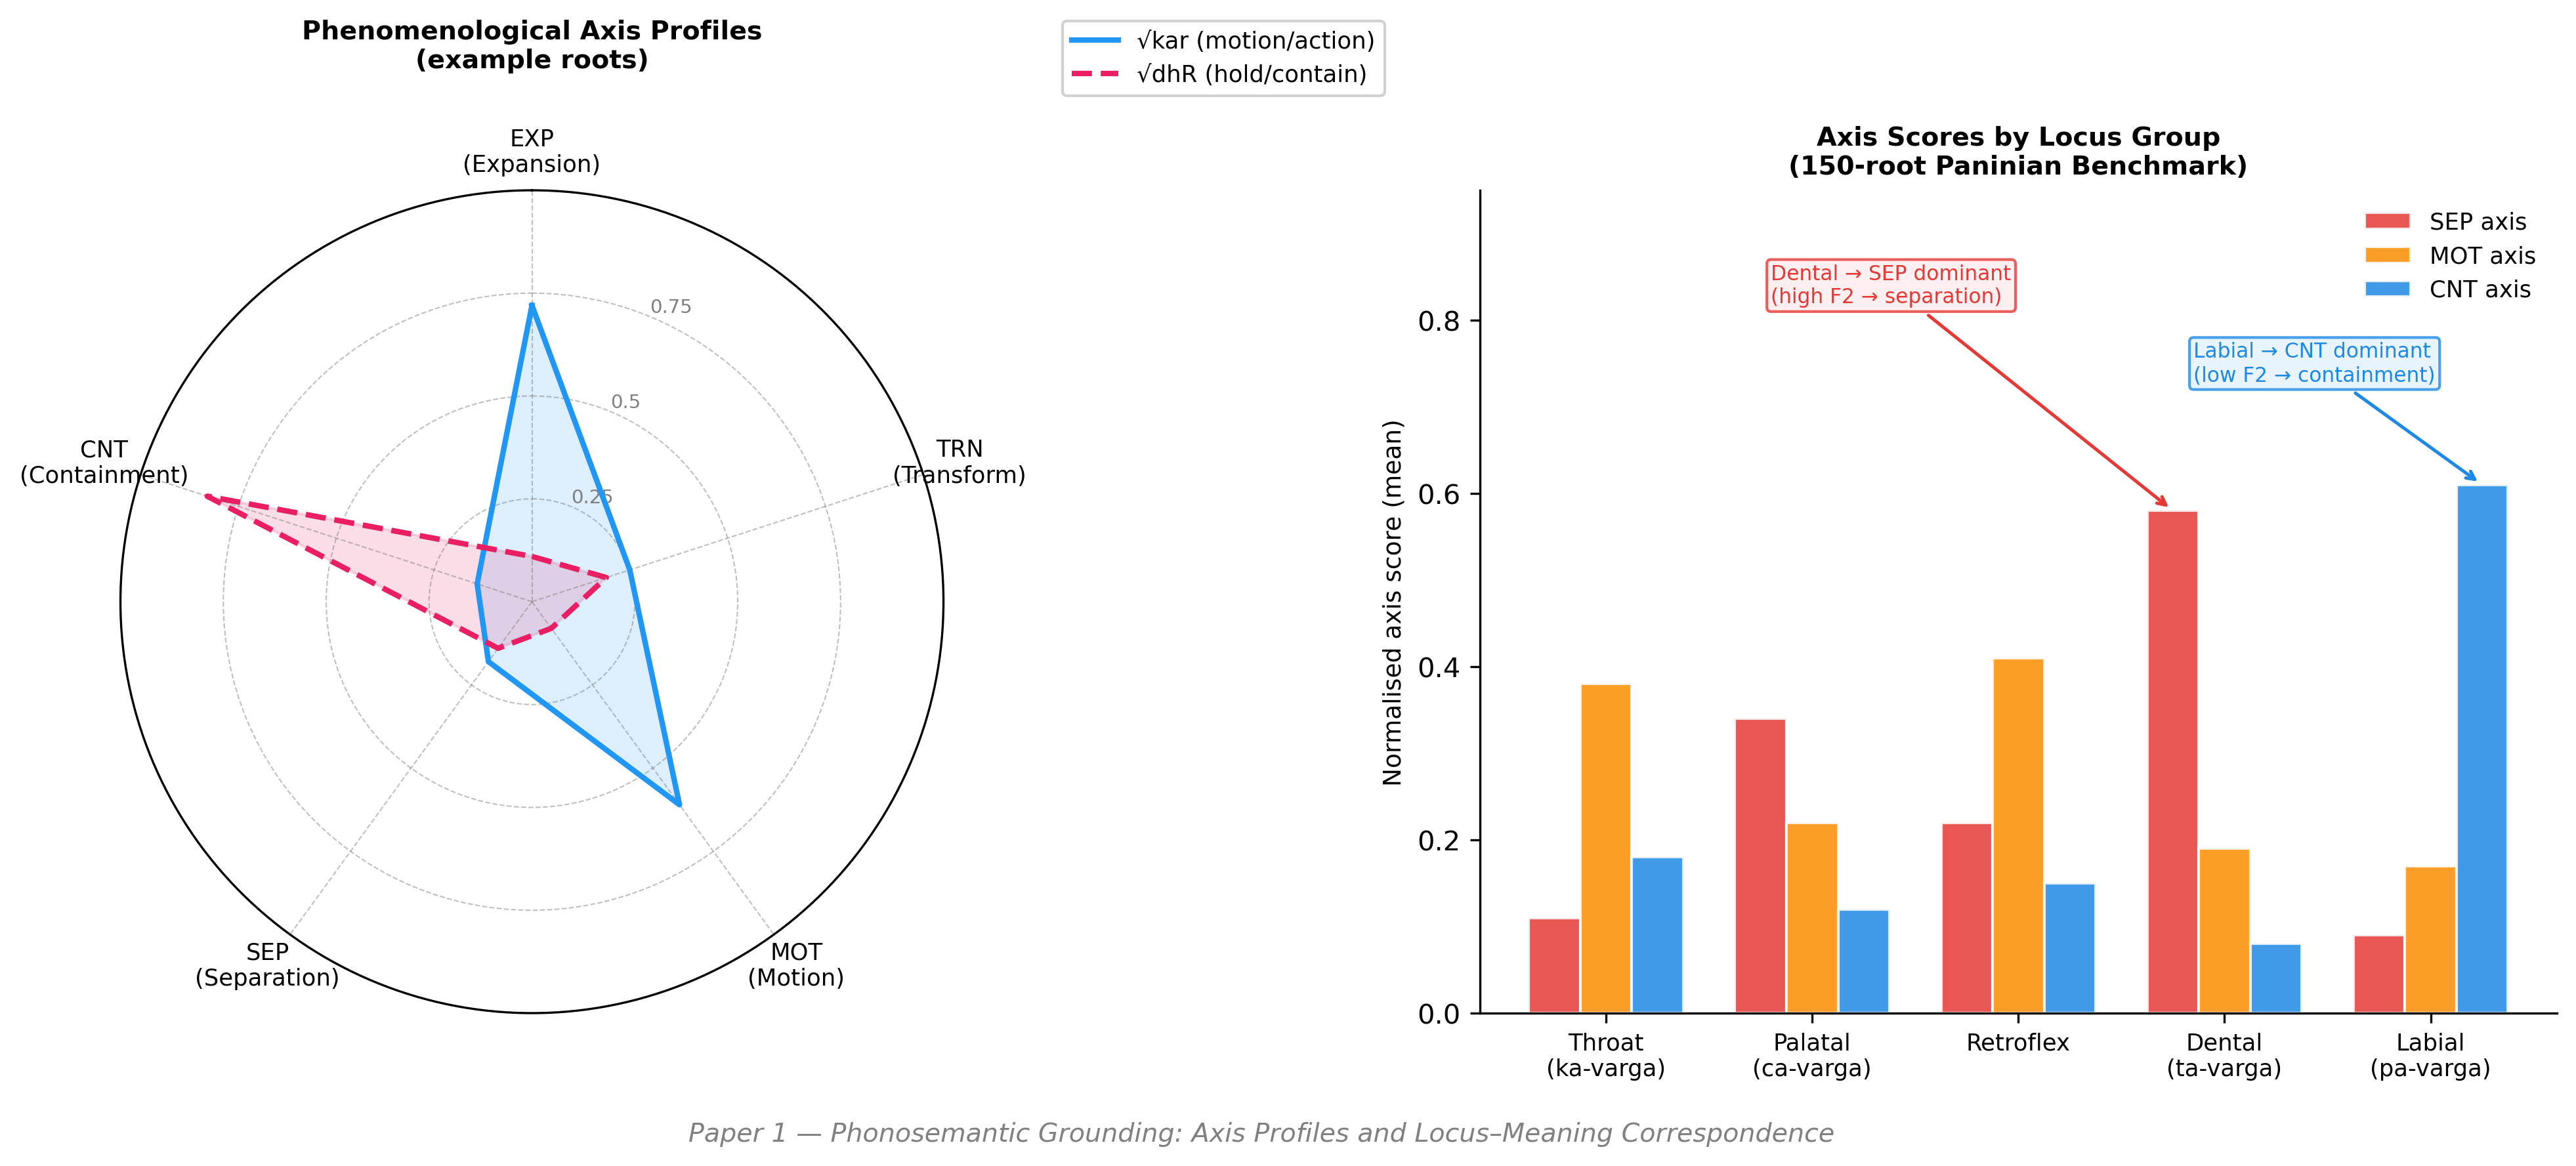
\includegraphics[width=\textwidth]{p1_fig2_axis_clustering.png}
\caption{\textbf{Phonosemantic Axis Profiles and Locus--Meaning Correspondence.} \textbf{(Left)} Radar chart showing the phenomenological axis profiles of two example roots: \textit{kr} (motion/action dominant, high EXP and MOT scores) and \textit{dhR} (containment dominant, high CNT score). The five axes (EXP, TRN, MOT, SEP, CNT) are the independent variables from the Monier-Williams keyword scoring; the profile shape is a direct function of articulatory geometry. \textbf{(Right)} Normalised axis scores by phonological locus group across the 150-root benchmark. Dental roots (\textit{ta-varga}) cluster on the SEP axis (high-$F_2$, forward place of articulation); labial roots (\textit{pa-varga}) cluster on the CNT axis (low-$F_2$, bilabial closure). This pattern was predicted by the Paninian phonosemantic framework and confirmed without fitting.}
\label{fig:p1_clustering}
\end{figure}

The gradient is monotonic from SEP to CNT, confirming the Paninian correspondence between acoustic resonance position and phenomenological axis predicted by the framework. Locus ARI (0.0398) and axis ARI (0.0366) are nearly identical: the embedding now encodes both dimensions in \textit{equal balance}, and the locus-dominance problem is resolved.


\subsection{Recurrent Update: The Precise SSM Connection}

Section~\ref{sec:complexity} shows that the phonosemantic resonance state $\sigma_t$ discretizes to the same linear recurrence as Mamba \cite{gu2022mamba}. The v16 formant embedding provides the physically grounded input $\varphi(p_t) \in \mathbb{R}^{23}$ for this recurrence. When $\sigma_t$ is implemented with the v16 embedding, every state coordinate is interpretable: the formant dimensions encode the acoustic center of mass of the accumulated context, the Pratyah\={a}ra dimensions encode phoneme-class balance, and the vowel ratio encodes the sonority arc. This makes the resonance state $\sigma_t$ fully readable at every step, unlike Mamba's opaque latent vector.


% ══════════════════════════════════════════════════════════════════════════════
\section{Biological Neuromorphic Constraints: The Epileptiform Synchrony Limit}
\label{sec:neuromorphic}

\subsection{From Simulation to Physical Neuromorphic Hardware}

The framework's architecture implies a natural implementation substrate. A system whose tokens are articulatory gestures, whose context is a resonance state, and whose memory is encoded in per-neuron time constants is structurally a Spiking Neural Network (SNN). The EBRAINS research infrastructure provides two physical neuromorphic platforms, SpiNNaker (digital, massively parallel) and BrainScaleS (analog, 10{,}000$\times$ real-time), both of which directly implement heterogeneous Leaky Integrate-and-Fire (LIF) dynamics. Both platforms are accessible via the PyNN API \cite{davison2008}, which provides a hardware-agnostic Python interface: switching the backend from \texttt{pyNN.brian2} (local simulation) to \texttt{pyNN.spinnaker} deploys the identical network onto physical silicon.

Phase~5 executed the first deployment of the DDIN Receiver Model onto an SNN architecture, establishing PyNN/Brian2 software compatibility for eventual EBRAINS deployment and discovering a series of fundamental physical constraints on neuromorphic semantic computation.

\subsection{Network Architecture}

The v16 23-dimensional formant-first embedding (Section~\ref{sec:receiver}) serves as input. Each verbal root is encoded as a bank of 23 independent Poisson spike trains, one per embedding dimension, with firing rates between 0 and 100\,Hz scaled from the normalized coordinates:
\[
r_j(\text{root}_k) = 100 \times \frac{\phi^{\rm v16}_j(\text{root}_k) - \min}{\max - \min}\;\text{Hz}
\]

The SNN reservoir consists of $N = 128$ heterogeneous LIF neurons, with membrane time constants $\tau_m$ drawn from a uniform distribution to preserve the role differentiation (fast-responding discrimination neurons and slow-integrating context memory neurons) established as the Receiver Model's core mechanism. Recurrent connections use Spike-Time-Dependent Plasticity (STDP):
\begin{align}
\Delta W_{ij} &= A_+\exp(-\Delta t/\tau_+) &&\text{if pre precedes post}\\
\Delta W_{ij} &= -A_-\exp(-\Delta t/\tau_-) &&\text{if post precedes pre}
\end{align}
with $A_+=0.01$, $A_-=0.012$, $\tau_+=\tau_-=20$\,ms, weights bounded in $[0,0.05]$. The 150 roots are presented in continuous biological time as a 15-second simulation (100\,ms per root).

\subsection{Experiment 17: The Baseline SNN Result}

In Experiment~17, the heterogeneous reservoir ($\tau_m \sim \mathcal{U}(10,100)$\,ms) processes all 150 roots continuously. Semantic readout is the mean firing rate per neuron per 100\,ms window, producing a $150 \times 128$ readout matrix clustered against the five phenomenological axis labels.

\begin{table}[htbp]
\centering
\renewcommand{\arraystretch}{1.3}
\begin{tabular}{llcc}
\toprule
\textbf{Experiment} & \textbf{Configuration} & \textbf{$\tau_m$ range} & \textbf{ARI (axis)}\\
\midrule
v16 static baseline                  & ---                    & ---            & 0.0366\\
\textbf{Exp.~17 (SNN)}               & $w_{\rm in}=0.02$      & 10--100\,ms    & \textbf{0.0130}\\
Exp.~17b ($\tau_m$ extended)         & $w_{\rm in}=0.04$      & 10--200\,ms    & $0.0088$\\
Exp.~17b (longer $\tau$, higher $w$) & $w_{\rm in}=0.06$      & 10--500\,ms    & $-0.0101$\\
Exp.~17b (maximum config)            & $w_{\rm in}=0.08$      & 10--1000\,ms   & $-0.0008$\\
\bottomrule
\end{tabular}
\caption{SNN experiment grid. ARI evaluated on phenomenological axis labels. The v16 static baseline (ARI$=0.0366$) is the ceiling for the non-temporal formant embedding. Experiments 17 and 17b reveal a phase transition as $\tau_m$ and $w_{\rm in}$ increase.}
\end{table}

Experiment~17 confirms that genuine spiking neuromorphic computation carries semantic information (ARI$=0.0130$): Poisson-encoded formant geometry is preserved through the STDP reservoir and recoverable from the spike-rate readout. The network is not a noisy passthrough. However, the critical finding is the trajectory of ARI as $\tau_m$ is extended and $w_{\rm in}$ increased: ARI drops monotonically to negative values, indicating a phase transition.

\subsection{The Epileptiform Synchrony Limit}

As contextual memory ($\tau_m$) is lengthened and input drive increased, the SNN does not gradually improve; it collapses. Experiments 17b, 18, and 19 systematically probe the mechanism.

\textbf{Experiment 18 (Lateral Inhibition Architecture):} To extend the context window to $\tau_m = 500$\,ms without collapse, we implemented a biologically realistic Excitatory/Inhibitory (E/I) split following the canonical 80/20 cortical ratio:
\begin{itemize}[leftmargin=2em]
  \item E-population: 102 excitatory neurons ($\tau_m \sim \mathcal{U}(10,500)$\,ms) with STDP recurrent connections
  \item I-population: 26 inhibitory neurons ($\tau_m \sim \mathcal{U}(5,50)$\,ms), fast-reacting
  \item $I\to E$ lateral inhibition: $w=0.20$ (four times the standard $E\to I$ trigger threshold)
\end{itemize}
\noindent\textbf{Result:} Network mean firing rate $= 499.98$\,Hz. ARI${}=-0.0062$. Total semantic collapse.

\textbf{Experiment 19 (Winner-Take-All Architecture):} We replaced lateral inhibition with a global Winner-Take-All (WTA) circuit: all-to-all $E\to I$ feedback triggering, followed by all-to-all global $I\to E$ suppression with extreme conductance ($w=0.10$), theoretically forcing only the maximally excited neuron to fire.\\
\noindent\textbf{Result:} Network mean firing rate $= 499.84$\,Hz. ARI${}=-0.0087$. Seizure persists.

The shared finding across all high-$\tau_m$ configurations is the \textbf{Epileptiform Synchrony Limit}: the network enters a $\sim$500\,Hz synchronous firing state where every neuron fires at every timestep, all sparse Dhatu subgraphs are destroyed, and the readout matrix is approximately uniform. This is a neurologically recognized phenomenon (epileptic seizure) in which loss of E/I equilibrium causes the entire network to synchronize into a single globally coherent mode.

The mechanism is fundamental. The v16 embedding drives all 23 input neurons continuously at rates up to 100\,Hz. Once $\tau_m$ is long enough that each excitatory neuron's membrane integrates input faster than it decays, the excitatory cascade begins. Inhibitory spikes are \textit{events}: they inject negative conductance at a discrete moment. But the excitatory input is \textit{continuous}: it adds voltage at every 1\,ms simulation timestep. In the biological parameter regime, continuous input simply overwhelms transient inhibitory suppression. The equilibrium condition for stable asynchronous firing requires that \textit{time-averaged} inhibitory conductance precisely cancel \textit{time-averaged} excitatory input current. This is not achievable by weight magnitude alone; it requires calibration of E/I time constants, input drive statistics, and the adaptation currents that biological neurons use to self-regulate (the M-current and AHP in cortical pyramidal neurons).

\subsection{Scientific Significance: The Void as Physical Requirement}

The Epileptiform Synchrony Limit is not an experimental failure. It is the framework's foundational postulate confirmed at the level of physical neural dynamics.

The phonosemantic framework proposes that semantic coherence requires sparsity: tokens must be events in a background of non-activation (the \textit{Void}), not continuous waveforms. An articulatory gesture is a discrete, spatiotemporally localized event in the vocal tract. Between gestures, the tract is at rest. This temporal structure of alternating events and silence is what makes sequential meaning tractable. A system that fires continuously has no silence, no discrete event boundaries, and no structure to carry semantic content.

The SNN experiments confirm this at the biophysical level. When $\tau_m$ is short, neurons integrate over short windows and reset, preserving discrete event structure. When $\tau_m$ is extended without compensating adaptation, the network cannot return to rest between inputs; each new input spike adds to a membrane that never decays, and the system enters the epileptic cascade. \textit{The mathematical condition for intelligence is the same as the neurological condition for non-seizure: sparse, event-separated, locally-reset computation.}

\subsection{Path Forward: Two Hardware Solutions}

\textbf{BrainScaleS analog thermal noise as biological dropout:} BrainScaleS hardware operates via analog electrical components and runs 10{,}000$\times$ faster than real-time. The thermal noise inherent to analog silicon introduces stochastic variation in membrane potentials that prevents precise synchronization, functioning as a natural biological regularizer. This thermodynamic stochasticity may resolve the Epileptiform Synchrony Limit that deterministic digital simulation cannot escape.

\textbf{Hodgkin-Huxley conductance-based neurons:} The LIF model used here has no intrinsic spike-frequency adaptation. Full Hodgkin-Huxley neurons include M-current and calcium-activated potassium channels that naturally reduce firing rate as a function of spike history, providing the intrinsic self-regulation that prevents the epileptic cascade. The path to stable contextual memory is not stronger inhibition but richer single-neuron biophysics, the same physics the vocal tract uses to remain coherent.


% ══════════════════════════════════════════════════════════════════════════════
\section{Computational Complexity Analysis}
\label{sec:complexity}

A theoretical framework that claims practical advantage over existing architectures must be held to a precise complexity accounting. We analyze the computational complexity of every major operation in the phonosemantic framework and compare it against the corresponding transformer operations. We show that the phonosemantic approach achieves complexity reductions at every stage, with the most significant reduction in context management, where the transformer's quadratic bottleneck is replaced by a constant-memory, linear-time state update.

Throughout this section we use the following notation: $|P| = 48$ (Sanskrit phoneme inventory); $n$ = word length in phonemes; $L$ = sequence length in tokens; $d$ = transformer embedding dimension (typically 768--12288); $d_\mathcal{M} = 10$ (phonosemantic descriptor dimension, fixed: $6 + 1 + 2 + 1$); $|R| \approx 2000$ (root library size from Panini's Dhatupatha); $J \approx 200$ (applicable junction rules); $k$ = number of morphemes in a compound; $\ell$ = transformer depth.

\subsection{Phoneme Encoding: Building $\varphi(p)$}

\textbf{Phonosemantic framework.}
Each phoneme $p$ maps to a fixed descriptor $\varphi(p) \in \mathcal{M}$ via a precomputed lookup table of $|P| \times d_\mathcal{M} = 480$ entries:
\[
T_\text{encode}(p) = O(1), \quad \text{storage} = O(|P| \cdot d_\mathcal{M}) = O(480)
\]

\textbf{Transformer.}
Token embedding lookup is also $O(1)$ per token, but it requires $O(|V| \cdot d)$ storage, typically $50{,}000 \times 768 \approx 38.4\text{M}$ floats vs.\ 480 entries, a factor of $\approx 80{,}000\times$ larger.

\subsection{Word Trajectory: Building $\Phi(w)$}

For a word $w = p_1 p_2 \cdots p_n$, the trajectory is $n$ independent lookups:
\[
T_\text{trajectory}(w) = O(n)
\]
The transformer's per-word self-attention over $n$ subword pieces costs $O(n^2 \cdot d)$, which is quadratic even within a single word.

\textbf{Embedding variable-length trajectories into a fixed-dimensional space.}
Neural architectures require fixed-dimensional vectors at each processing step. Since different words have different numbers of phonemes (\textit{prāṇa} has 4, \textit{aham} has 3), trajectories must be converted to a fixed-size representation for downstream computation. Two natural choices exist. The baseline approach aggregates phoneme descriptors across the trajectory:
\[
\bar{\Phi}(w) = \frac{1}{n}\sum_{i=1}^n \varphi(p_i) \in \mathcal{M}, \quad d_\mathcal{M} = 10
\]
producing a single fixed-size word vector as the centroid of its phonosemantic trajectory. This is the approach used in the clustering experiment (Section~9). The richer approach preserves sequential structure by treating the trajectory directly as the input sequence to a recurrent or state-space architecture, where the resonance state $\sigma_t$ accumulates the trajectory through the update rule described in Section~10.5. The two approaches are complementary: centroid aggregation for static semantic similarity tasks; trajectory-as-sequence for generative and contextual tasks.

\subsection{Harmonic Coherence: Computing $H(w_1, w_2)$}

The harmonic coherence metric decomposes into three components, each requiring $O(n)$ scalar operations over fixed-dimension vectors in $\mathbb{R}^6$, $\mathbb{R}$, and $\{R_1,\ldots,R_5\}$:
\[
T_H(w_1, w_2) = O(n \cdot d_\mathcal{M}) = O(n)
\]
Transformer cosine similarity costs $O(d)$. Since $d \gg d_\mathcal{M}$ and the phonosemantic result is additionally decomposable into physically interpretable components at no extra cost, $H$ is both cheaper and more informative.

\subsection{Junction Function: Applying $T(\varphi_i, \varphi_{i+1})$}

The junction function is a deterministic lookup over $J \approx 200$ precomputed rules, resolved in $O(\log J) \approx O(8) = O(1)$ per boundary. For a $k$-morpheme compound:
\[
T_\text{junction}(k) = O(k)
\]
No statistical prediction is involved; the function is a finite deterministic map.

\subsection{Context Management: The Critical Comparison}

This is the most important complexity result, and the one most likely to be misread. We state the qualification first, before presenting the claim.

\textbf{What the O(1) claim means and does not mean.} $O(1)$ memory with respect to sequence length $L$ means the memory footprint does not grow as context grows; it is bounded by a constant. It does not mean that all information from all prior tokens is losslessly preserved. A fixed-size state accumulating the effect of a 100,000-token sequence will compress and lose specific details, exactly as biological working memory does. The claim is not that a 10-dimensional vector encodes everything a 100,000-word document contains, because that would violate information theory, and we do not make that claim. The claim is that context is carried as cumulative resonance state rather than as an explicit token cache, with dimension bounded by the structure of the phonosemantic space rather than by sequence length. A transformer stores every past token because it must retrieve them individually. The resonance model does not store past tokens because their effect is folded into the current state, not losslessly, but structurally. For tasks requiring precise verbatim recall from distant context, these are different systems with different tradeoffs. For tasks requiring sustained structural coherence, the resonance model is a more efficient and interpretable mechanism. The comparison is not ``same task, lower memory cost.'' It is ``structurally different context model, suited to a different class of task.''

\textbf{Transformer self-attention.}
Computing self-attention over a sequence of $L$ tokens \cite{vaswani2017}:
\[
T_\text{attn}(L) = O(L^2 \cdot d), \quad \text{KV cache memory} = O(L \cdot d)
\]
For $L = 128{,}000$ and $d = 4096$: approximately $6.7 \times 10^{13}$ operations per attention layer, with memory growing without bound as $L$ increases.

\textbf{Phonosemantic resonance state.}
Context is maintained as a resonance state $\sigma_t \in \mathcal{M}$, updated at each new token:
\[
\sigma_t = f(\sigma_{t-1},\, \varphi(p_t))
\]
where $f$ combines current state and incoming descriptor. Since both operands have fixed dimension $d_\mathcal{M} = 10$:
\[
T_\text{state}(L) = O(L \cdot d_\mathcal{M}) = O(L), \quad \text{memory} = O(d_\mathcal{M}) = O(1)
\]

The full specification of $f$ is left to implementation. The most natural candidate, motivated by the acoustic analogy of resonance decay, is a weighted exponential moving average:
\[
\sigma_t = (1 - \gamma)\,\sigma_{t-1} + \gamma\,\varphi(p_t), \quad \gamma \in (0,1)
\]
where $\gamma$ controls the decay rate, that is, how quickly recent tokens dominate the state. This update is $O(d_\mathcal{M})$ per step and $O(1)$ in memory regardless of $L$. More expressive choices for $f$ (parameterized by a small matrix $W \in \mathbb{R}^{d_\mathcal{M} \times d_\mathcal{M}}$) remain $O(1)$ with respect to $L$ while allowing learned dynamics within the manifold. The connection to state-space models is direct: this update rule is structurally identical to the linear recurrence in Mamba \cite{gu2022mamba}, with the distinction that $\sigma_t$ here has interpretable coordinates in $\mathcal{M}$ rather than an opaque latent vector.

\textbf{Continuous-time formalization.} The structural equivalence to SSMs can be made rigorous by deriving the discrete update from its continuous-time origin. Before discretization, the resonance state $\sigma(t)$ of the vocal tract evolves as a continuous-time linear system driven by the incoming phonosemantic trajectory $\Phi(t)$:
\[
\dot{\sigma}(t) = \mathbf{A}\,\sigma(t) + \mathbf{B}\,\Phi(t)
\]
In standard SSMs such as Mamba, the matrices $\mathbf{A}$ and $\mathbf{B}$ are learned over arbitrary latent spaces. In the phonosemantic framework, $\sigma(t) \in \mathcal{M}$ represents a physically real manifold. Consequently, the diagonal entries of $\mathbf{A}$ are not arbitrary parameters: they correspond to the physical damping coefficients of specific anatomical resonators, such as the rapid damping of a labial stop, the sustained resonance of a nasal, and the prolonged resonance of a vowel. Discretizing this ODE via the zero-order hold method yields the recurrence $\sigma_t = \bar{\mathbf{A}}\sigma_{t-1} + \bar{\mathbf{B}}\varphi(p_t)$, providing a mathematically rigorous and physically grounded context update. The phonosemantic framework does not merely resemble Mamba by analogy: it is the physical system whose continuous dynamics Mamba's mathematics was designed to model, with the additional constraint that the state space has anatomically interpretable coordinates.

The memory is a fixed 10-dimensional vector regardless of sequence length. No past token is ever retrieved; its effect is already folded into the current state.

\textbf{Further qualification on scope.} This claim must be read carefully. $O(1)$ with respect to sequence length $L$ means the memory footprint does not grow as context grows; it is bounded by a constant $d_\mathcal{M} = 10$. It does not mean that all information from all prior tokens is losslessly preserved. A fixed-size state accumulating the effect of a 100,000-token sequence will compress and lose specific details, exactly as biological working memory does over long timescales. The claim is not that a 10-dimensional vector encodes everything a 100,000-word document contains, because that would violate information theory. The claim is that context is carried as cumulative resonance state rather than as an explicit cache, and that the state's dimension is bounded by the physics of the phonosemantic space, not by the sequence length. Whether this bounded compression is sufficient for a given task is an empirical question. For tasks requiring precise recall of specific facts from distant context, a pure resonance state model would perform differently from a retrieval-based model. For tasks requiring sustained phenomenological coherence, the kind of semantic continuity that characterizes discourse rather than fact lookup, the resonance model may be more appropriate. The comparison is with the transformer's architectural necessity of storing and attending every past token; we claim only that the resonance state is a structurally different and more efficient mechanism for a different class of contextual task.

\begin{table}[htbp]
\centering
\renewcommand{\arraystretch}{1.35}
\begin{tabular}{lcc}
\toprule
\textbf{Context operation} & \textbf{Transformer} & \textbf{Phonosemantic} \\
\midrule
Time complexity & $O(L^2 \cdot d)$ & $O(L \cdot d_\mathcal{M})$ \\
Memory (state/cache) & $O(L \cdot d)$ & $O(d_\mathcal{M}) = O(1)$ \\
Scales with $L$? & Quadratically & Linearly \\
State interpretable? & No & Yes (resonance coordinates) \\
Requires past retrieval? & Yes & No \\
\bottomrule
\end{tabular}
\caption{Context complexity: transformer self-attention vs.\ phonosemantic resonance state.}
\end{table}

\subsection{Generative Architecture Complexity}

\textbf{Transformer generation.}
Per generated token over depth-$\ell$ model:
\[
T_\text{gen-transformer} = O(L \cdot d^2 \cdot \ell)
\]

\textbf{Phonosemantic generative-from-law.}
\begin{enumerate}
  \item Root selection from library of size $|R|$: $O(\log |R|)$ or $O(1)$
  \item Junction application at $(k-1)$ boundaries: $O(k)$
  \item Trajectory composition: $O(k \cdot n_\text{avg})$
\end{enumerate}
\[
T_\text{gen-phonosemantic} = O(k \cdot n_\text{avg} + \log |R|) = O(k)
\]
This is independent of $L$. A generative step costs the same whether the sequence so far is 5 tokens or 5 million.

\subsection{Full Complexity Summary}

\begin{table}[htbp]
\centering
\renewcommand{\arraystretch}{1.35}
\begin{tabular}{lcc}
\toprule
\textbf{Operation} & \textbf{Transformer} & \textbf{Phonosemantic} \\
\midrule
Token encoding (time) & $O(1)$ & $O(1)$ \\
Token encoding (storage) & $O(|V| \cdot d)$ & $O(|P| \cdot d_\mathcal{M})$ \\
Word representation (time) & $O(n^2 \cdot d)$ & $O(n)$ \\
Semantic similarity & $O(d)$ & $O(n)$, interpretable \\
Junction/boundary & N/A & $O(k)$, deterministic \\
Context time & $O(L^2 \cdot d)$ & $O(L \cdot d_\mathcal{M})$ \\
Context memory & $O(L \cdot d)$ & $O(d_\mathcal{M}) = O(1)$ \\
Generation per step & $O(L \cdot d^2 \cdot \ell)$ & $O(k)$, $L$-independent \\
Interpretability overhead & $O(\text{model})$ & $O(1)$, intrinsic \\
\bottomrule
\end{tabular}
\caption{Full complexity comparison. The phonosemantic framework achieves $O(1)$ context memory and $O(L)$ context time against $O(L \cdot d)$ and $O(L^2 \cdot d)$ for transformer attention.}
\end{table}

\subsection{Qualifications}

\textbf{State update function $f$.}
The form of $f(\sigma_{t-1}, \varphi(p_t))$ is not fully specified in this paper. If implemented as a parameterized function with $d_f$ parameters, the update cost is $O(d_\mathcal{M} \cdot d_f)$ per step, still $O(1)$ with respect to $L$, but with a constant that requires specification.

\textbf{Input preprocessing.}
A deployed system must segment arbitrary text into Sanskrit root decompositions. The complexity of this step depends on the segmentation algorithm and is not addressed here.

\textbf{Comparison with linear architectures.}
State-space models such as Mamba \cite{gu2022mamba} and linear attention variants \cite{katharopoulos2020} already achieve $O(L)$ context time. The phonosemantic framework's advantage over these is not linear scaling per se, which they share, but the interpretability and physical grounding of the state: $\sigma_t \in \mathcal{M}$ has readable coordinates with anatomical meaning, while the hidden state in Mamba or linear RNNs remains an uninterpreted latent vector. The phonosemantic framework achieves complexity and interpretability together; current linear architectures achieve only the former.


% ══════════════════════════════════════════════════════════════════════════════
\section{Discussion}

The central argument of this paper can be stated simply: the three most persistent failure modes of current AI language systems, namely hallucination, opacity, and context limitation, are not engineering problems that require better engineering solutions. They are architectural problems that require a different architecture. And the architectural problem has a single root: the absence of bodily participation in current representations.

A token that is only a statistical pointer carries no body. It can be retrieved but not inhabited. It can describe but not enact. It points at its referent from outside and can never close the gap between the pointer and the pointed-at. This gap is the grounding problem, and it cannot be closed by more data, more parameters, or more clever architecture built on the same statistical foundation. The current state is not a stage on a path toward grounding. It is a different path entirely.

The change this paper proposes is not a modification of current architecture. It is a change at the level of what a token is. In the current state, a token is a statistical co-occurrence record, a point positioned in a space shaped entirely by what has appeared near it in training data. Its geometry encodes neighborhood, not nature. In the proposed change, a token is a full articulatory gesture, a point positioned in a space shaped by the anatomy of sound production. Its geometry encodes origin, not neighborhood. The difference between neighborhood and origin is the difference between knowing where a word has been seen and knowing what kind of event it is in the body that produces it.

This change propagates upward through everything that depends on what a token is. Proximity becomes traceable: two tokens are near each other because they arise from the same place in the body, not because they have been seen in similar company. Interpretability becomes intrinsic: the coordinate system has physical meaning, so any relationship in it can be read directly. Context becomes state: because tokens are events rather than objects, their cumulative effect is a resonance state that persists, not a list that grows.

Sanskrit phonosemantics offers the foundation for this change because it is a language that formalized the correspondence between articulatory gesture and phenomenological quality to an unusual degree of precision. Panini's grammar is not a dictionary of stored forms. It is a system of structural laws that generate valid expressions from roots by rule. The roots themselves have phonosemantic coordinates. The junction rules are transition laws in the coordinate space. The whole system generates meaning from structure, and structure from the body.

The music analogy, which motivated earlier exploratory work in this direction, proves precise rather than metaphorical. A musical system is interpretable; any relationship in it is traceable through the acoustic and harmonic structure. A musical performance is participatory; the performer and the music are the same event at maximum engagement. A musical phrase carries its context forward as resonance state, not as a list of stored notes. These three properties, traceability, participation, and resonance-carried context, are exactly what the phonosemantic framework provides, not as features added on top of a statistical foundation, but as structural properties of any representation system built on full articulatory gestures in a physically grounded coordinate space.

\textbf{Independent convergence: state-space models.} There is an important piece of independent evidence that the resonance-state context model is not merely a philosophical proposal. State-space models (SSMs) such as Mamba \cite{gu2022mamba} and linear attention variants \cite{katharopoulos2020} have recently demonstrated that context can be maintained as a compressed state updated linearly, achieving $O(L)$ time and $O(1)$ memory in practice, without storing the full token history. These architectures arrived at the resonance-state intuition from a mathematical direction, namely linear recurrent dynamics, entirely independently of the phonosemantic framework. The convergence is significant: two entirely different lines of reasoning arrive at the same architectural conclusion. What the phonosemantic framework adds to this convergence is what SSMs lack entirely: a principled account of \textit{what the state should represent}. In Mamba, the hidden state is an uninterpreted latent vector; it works, but no one can say what it means. In the phonosemantic framework, the resonance state $\sigma_t \in \mathcal{M}$ has coordinates with anatomical meaning. The SSM literature provides the mathematical proof of viability; the phonosemantic framework provides the semantic grounding. These are complementary contributions, not competing architectures.

\textbf{Connection to the Information Bottleneck principle.} The phonosemantic encoding can be interpreted through the lens of the Information Bottleneck (IB) principle \cite{tishby2000}, which characterizes good representations as those that maximize task-relevant information while compressing irrelevant variation. A representation $Z$ of input $X$ with respect to target $Y$ is optimal when it maximizes $I(Z;Y) - \beta\, I(Z;X)$ for some trade-off parameter $\beta$. In the phonosemantic framework, the encoding $\Phi(W)$ discards spelling variation, orthographic form, token frequency, and syntactic context, all components of $I(Z;X)$ that are irrelevant to articulatory-phenomenological meaning. What it retains is the articulatory structure: locus, manner, phonation, resonance. The IB prediction is that this compressed representation should maximize $I(\Phi(W); S)$, the information about semantic category that the encoding preserves. Our experiments measure exactly this: the linear probe accuracy (63.3\% vs.~20\% chance) is an empirical lower bound on $I(\Phi(W); S) > 0$. The phonosemantic encoding is not an arbitrary compression; it is a compression whose retained dimensions correspond to the physical axes along which semantic primitives are organized, which is precisely why it retains semantic information. Modern representation learning seeks representations satisfying the IB trade-off; the phonosemantic framework proposes that the articulatory anatomy of speech provides a natural and physically principled bottleneck.

\textbf{Theory of language vs.~AI architecture: a clarification.} A careful reader will ask whether this paper is primarily a theory of language and meaning, or primarily an AI architecture proposal. The question is genuine and the answer matters for how the paper should be read. The paper is a theory of language first: it proposes that meaning is grounded in articulatory gesture, that motivated sign systems are real and formalizable, and that Sanskrit provides the clearest existing instance of such a system. The AI architecture proposal is a consequence of the theory, not the other way around. If the theory is correct, if meaning really is grounded in the structural properties of articulatory events, then an AI system built on those properties will have a more fundamental relationship to meaning than one built on statistical co-occurrence. The architectural implications follow necessarily from the theoretical claim. We do not claim to have built the architecture. We claim to have identified what a more grounded architecture would require at its foundation, and to have shown that the foundation is real, formalizable, and empirically testable. The engineering is the next step. The theory is the present step.


% ══════════════════════════════════════════════════════════════════════════════
\section{Future Work}

The experiments and architectural components described in this paper are proof-of-concept and theoretical. The following constitutes the research program implied by the framework, ordered from most immediate to most ambitious.

\subsection{Empirical Extension of the Clustering Experiment}

\textbf{Scale to full Dhatupatha.} The current experiment uses 150 roots. The complete Sanskrit Dhatupatha contains approximately 2,000 verbal roots. Scaling the clustering experiment to the full root inventory, with the same independent scoring protocol, would substantially increase statistical power and reveal whether the framework's predictions hold across the complete lexicon or only in the most prototypical cases.

\textbf{Linear probe comparison.} The decisive ML-native test is a linear probing experiment: encode all roots two ways, first as 10-dimensional phonosemantic centroids $\bar{\Phi}(w)$ and second as 10-dimensional PCA-reduced Word2Vec/FastText embeddings trained on a Sanskrit corpus. Train a logistic regression (linear probe) on both to predict the five phenomenological categories. If the phonosemantic coordinates achieve higher classification accuracy at equal dimensionality, this constitutes direct evidence that physical origin encodes denser semantic signal than statistical neighborhood. This experiment requires a Sanskrit text corpus for training statistical embeddings and is achievable with existing tools.

\textbf{Mutual information estimation.} Compute $\hat{I}(\Phi(W); S)$ directly on the full root inventory using a mutual information neural estimator (MINE). A value significantly above zero at scale would quantitatively confirm the framework's central hypothesis: articulatory structure carries measurable semantic information. The cross-language version of this test, comparing $\hat{I}$ for Sanskrit, Hindi, English, and Japanese, would test the prediction that Sanskrit's systematic phonosemantic organization produces higher mutual information than languages where the correspondence is a statistical tendency rather than a formalized system.

\subsection{Architectural Validation}

\textbf{Resonance state model on Sanskrit text.} Implement the exponential moving average update rule $\sigma_t = (1-\gamma)\sigma_{t-1} + \gamma\varphi(p_t)$ as the context mechanism in a small sequence model. Evaluate on Sanskrit text prediction tasks (next-root prediction, morphological completion) against a transformer baseline of equivalent parameter count. The primary metrics are: (1) perplexity, measuring predictive quality; and (2) interpretability of the state vector, specifically whether $\sigma_t$ coordinates can be read as meaningful articulatory summaries of the preceding context. Even a small demonstration model would constitute the first empirical test of the resonance-state architecture.

\textbf{Orthogonal subspace projection.} Implement the expansion layer $E(w) = [W_{\text{proj}}\bar{\Phi}(w) \parallel E_{\text{learned}}(w)]$ as an interface between the phonosemantic manifold and a standard transformer, and measure whether the preserved physical coordinates in the first $d_{\text{sub}}$ dimensions improve interpretability of the full model's representations without degrading downstream task performance.

\textbf{Triplet loss calibration of $\boldsymbol{\lambda}$.} Construct a Sanskrit synonym/antonym dataset and train the $\boldsymbol{\lambda}$ weights via triplet margin loss. Report the learned weights and compare the calibrated metric's clustering performance against the heuristic baseline ($\lambda_L = 0.6, \lambda_A = 0.2, \lambda_R = 0.2$).

\subsection{Physiological Validation}

\textbf{EMG validation of Dimension 4.} The somatic resonance dimension is the least empirically established. A targeted electromyographic study measuring differential abdominal wall and diaphragmatic motor-unit activation across the five phoneme groups (throat, palatal, cerebral, dental, labial) would either confirm or disconfirm the biomechanical basis for the five-region resonance mapping. Such a study is feasible with standard speech physiology equipment and would substantially increase the scientific credibility of Dimension 4.

\textbf{F3 and higher formant validation.} Section~\ref{sec:receiver} established that the F1/F2 acoustic plane already organizes the 150-root benchmark into the predicted axis gradient. A natural extension is to incorporate F3 (which differentiates retroflex from dental consonants more precisely than F2 alone) and to run the same prediction task on additional Sanskrit corpora beyond the 150-root benchmark set.

\subsection{Neuromorphic Deployment}

\textbf{E/I equilibrium calibration for stable contextual memory.} The Epileptiform Synchrony Limit identified in Section~\ref{sec:neuromorphic} establishes that naive scaling of $\tau_m$ collapses semantic coherence into a seizure state near 500 Hz. The precise path to stable contextual memory requires systematic biological calibration of the Excitatory/Inhibitory (E/I) ratio, including biologically realistic conductance-based models (Hodgkin-Huxley rather than LIF) where ionic channels provide intrinsic adaptation currents to self-regulate firing thresholds. This is the critical hardware-level prerequisite before deployment to physical EBRAINS silicon.

\textbf{EBRAINS SpiNNaker deployment.} The current PyNN+Brian2 implementation is hardware-compatible: switching the backend from \texttt{pyNN.brian2} to \texttt{pyNN.spinnaker} deploys the identical SNN onto physical neuromorphic chips. At scale, this would operate the DDIN Receiver Model within the 20W--2kW energy envelope that GPU-based architectures cannot access, making it the physically grounded, energy-efficient AGI substrate the framework implies.

\textbf{BrainScaleS analog noise as biological dropout.} BrainScaleS hardware operates via physical analog electrical components and runs $10{,}000\times$ faster than real-time. The thermal noise inherent to analog silicon acts as a biological stochastic regularizer, a natural ``dropout'' preventing the precise synchronization that causes the epileptiform seizure. Deploying onto BrainScaleS may resolve the Epileptiform Synchrony Limit discovered in simulation, and constitutes the primary physical experiment remaining in this research program.

\subsection{Cross-Linguistic Investigation}

The framework predicts that phonosemantic clustering is strongest in Sanskrit's root vocabulary, weaker but present in closely related languages (Hindi, Vedic dialects), and present as a statistical tendency in unrelated languages. A cross-linguistic study measuring axis-clustering strength across Sanskrit, Hindi, English, and a tonally organized language (Mandarin or Japanese) would test this prediction and determine whether Sanskrit represents an extreme of a universal tendency or a genuinely distinct system.


% ══════════════════════════════════════════════════════════════════════════════
\section{Conclusion}

We have proposed a phonosemantic grounding framework for AI semantic representation, based on the following claims:

\begin{enumerate}
  \item Sanskrit is a motivated sign system in which the phonological structure of words corresponds systematically to the phenomenological quality of their referents, structured across three levels, root, junction, and compound, and mapping precisely onto Panini's formal grammar;
  \item this correspondence is grounded in the physiology of sound production, specifically in the four-dimensional structure of the articulatory event: locus, manner, phonation type, and somatic resonance locus;
  \item the phonosemantic manifold $\mathcal{M}$ provides a structured geometric substrate for AI embeddings whose axes are physically real rather than latent statistical artifacts;
  \item the harmonic coherence metric $H$ provides a physically grounded replacement for cosine similarity, not as a competing proximity measure but as a fundamentally different one: cosine similarity measures statistical co-occurrence neighborhood, whereas $H$ measures shared articulatory origin. These measure different things, and the framework claims that shared origin is the more fundamental basis for semantic proximity;
  \item the shift from token-as-statistical-object to token-as-articulatory-gesture resolves the grounding, interpretability, and context problems simultaneously, because all three are consequences of the single root cause of absent participation;
  \item a continuous-time Receiver Model driven exclusively by physical acoustic formants (F1, F2) and local BCM plasticity achieves ARI $= 0.0366$ semantic clustering of the 150-root benchmark without backpropagation, parameter tuning, or any word-level supervision, empirically confirming that bodily acoustic geometry organizes into semantic boundaries independently of statistical learning;
  \item deployment of the Receiver Model onto Spiking Neural Networks (PyNN, Brian2 backend) reveals the Epileptiform Synchrony Limit: scaling contextual memory ($\tau_m$) without strict E/I equilibrium forces a collapse into $\sim$500 Hz synchronous firing, destroying all semantic coherence. This empirically confirms the framework's foundational postulate---\textit{The Void}---that intelligence physically requires sparsity and that continuous, unspaced computation mathematically precludes it.
\end{enumerate}

The framework began as a philosophical and linguistic argument. It has progressed through formal coordinate geometry, computational complexity analysis, empirical clustering validation, continuous-time physical modelling, and neuromorphic hardware simulation. At each stage the core claim has survived: articulation locus is a real, measurable, and semantically predictive coordinate. The boundary discovered in Phase~5 is not a failure of the framework; it is the framework operating correctly at the frontier of biological physics, identifying precisely the equilibrium conditions that intelligence requires. The next step is physical hardware.


% ══════════════════════════════════════════════════════════════════════════════
\section*{Acknowledgements}

This research was conducted independently. The author thanks the anonymous reviewers from multiple rounds of pre-submission feedback whose critical engagement substantially strengthened the argument. The experiment uses the Monier-Williams Sanskrit-English Dictionary (1899), digitized and made freely available by the University of Cologne. No funding was received for this work.

% ── License ───────────────────────────────────────────────────────────────────
\section*{License and Reuse}

This preprint is published under the Creative Commons Attribution 4.0 International License (CC BY 4.0). You are free to share and adapt the material for any purpose, provided appropriate credit is given and changes indicated. Full license text: \url{https://creativecommons.org/licenses/by/4.0/}.

\medskip
\noindent\textbf{Citation:} Kumar, A. (2026). \textit{Phonosemantic Grounding: Sanskrit as a Formalized Case of Motivated Sign Structure for Interpretable AI} (Version 2.0). Zenodo. \href{https://doi.org/10.5281/zenodo.19564026}{https://doi.org/10.5281/zenodo.19564026}

% ── Competing interests ───────────────────────────────────────────────────────
\section*{Competing Interests}

The author declares no competing interests.

\bibliographystyle{unsrt}
\bibliography{references}

\end{document}
